%# -*- coding: utf-8-unix -*-
%%==================================================
%% thesis.tex
%%==================================================

% 双面打印
\documentclass[master, fontset=adobe, openany, oneside, zihao=-4]{sjtuthesis}
% \documentclass[bachelor, fontset=adobe, openany, oneside, zihao=-4, submit]{sjtuthesis} 
% \documentclass[master, adobefonts, review]{sjtuthesis} 
% \documentclass[%
%   bachelor|master|doctor,	% 必选项
%   fontset=adobe|windows,  	% 只测试了adobe
%   oneside|twoside,		% 单面打印,双面打印(奇偶页交换页边距,默认)
%   openany|openright, 		% 可以在奇数或者偶数页开新章|只在奇数页开新章(默认)
%   zihao=-4|5,, 		% 正文字号:小四、五号(默认)
%   review,	 		% 盲审论文,隐去作者姓名、学号、导师姓名、致谢、发表论文和参与的项目
%   submit			% 定稿提交的论文,插入签名扫描版的原创性声明、授权声明 
% ]

% 逐个导入参考文献数据库
\addbibresource{bib/thesis.bib}
% \addbibresource{bib/chap2.bib}

\begin{document}

%% 无编号内容:中英文论文封面、授权页
%# -*- coding: utf-8-unix -*-
\title{模拟集成电路符号化低阶模型自动生成方法与应用}
\author{胡翰彬}
\advisor{施国勇\quad{}教授}
\defenddate{2016年1月}
\school{上海交通大学}
\institute{微纳电子学系}
\studentnumber{1132109003}
\major{电子科学与技术}
\funding{本研究由国家自然科学基金(项目号 61176129, 61474145)资助。}

\englishtitle{Automatic Generation Method of Low-order Models for Analog Integrated Circuits with Applications}
\englishauthor{Hanbin Hu}
\englishadvisor{Prof. Guoyong Shi}
\englishschool{Shanghai Jiao Tong University}
\englishinstitute{Dept. of Micro-Nano Electronics}
\englishmajor{Electronic Science and Technology}
\englishdate{Jan, 2016}
\englishdegree{Master of Science}


\maketitle

\makeenglishtitle

\makeatletter
\ifsjtu@submit\relax
	
\includepdf{pdf/original.pdf}
	\cleardoublepage
	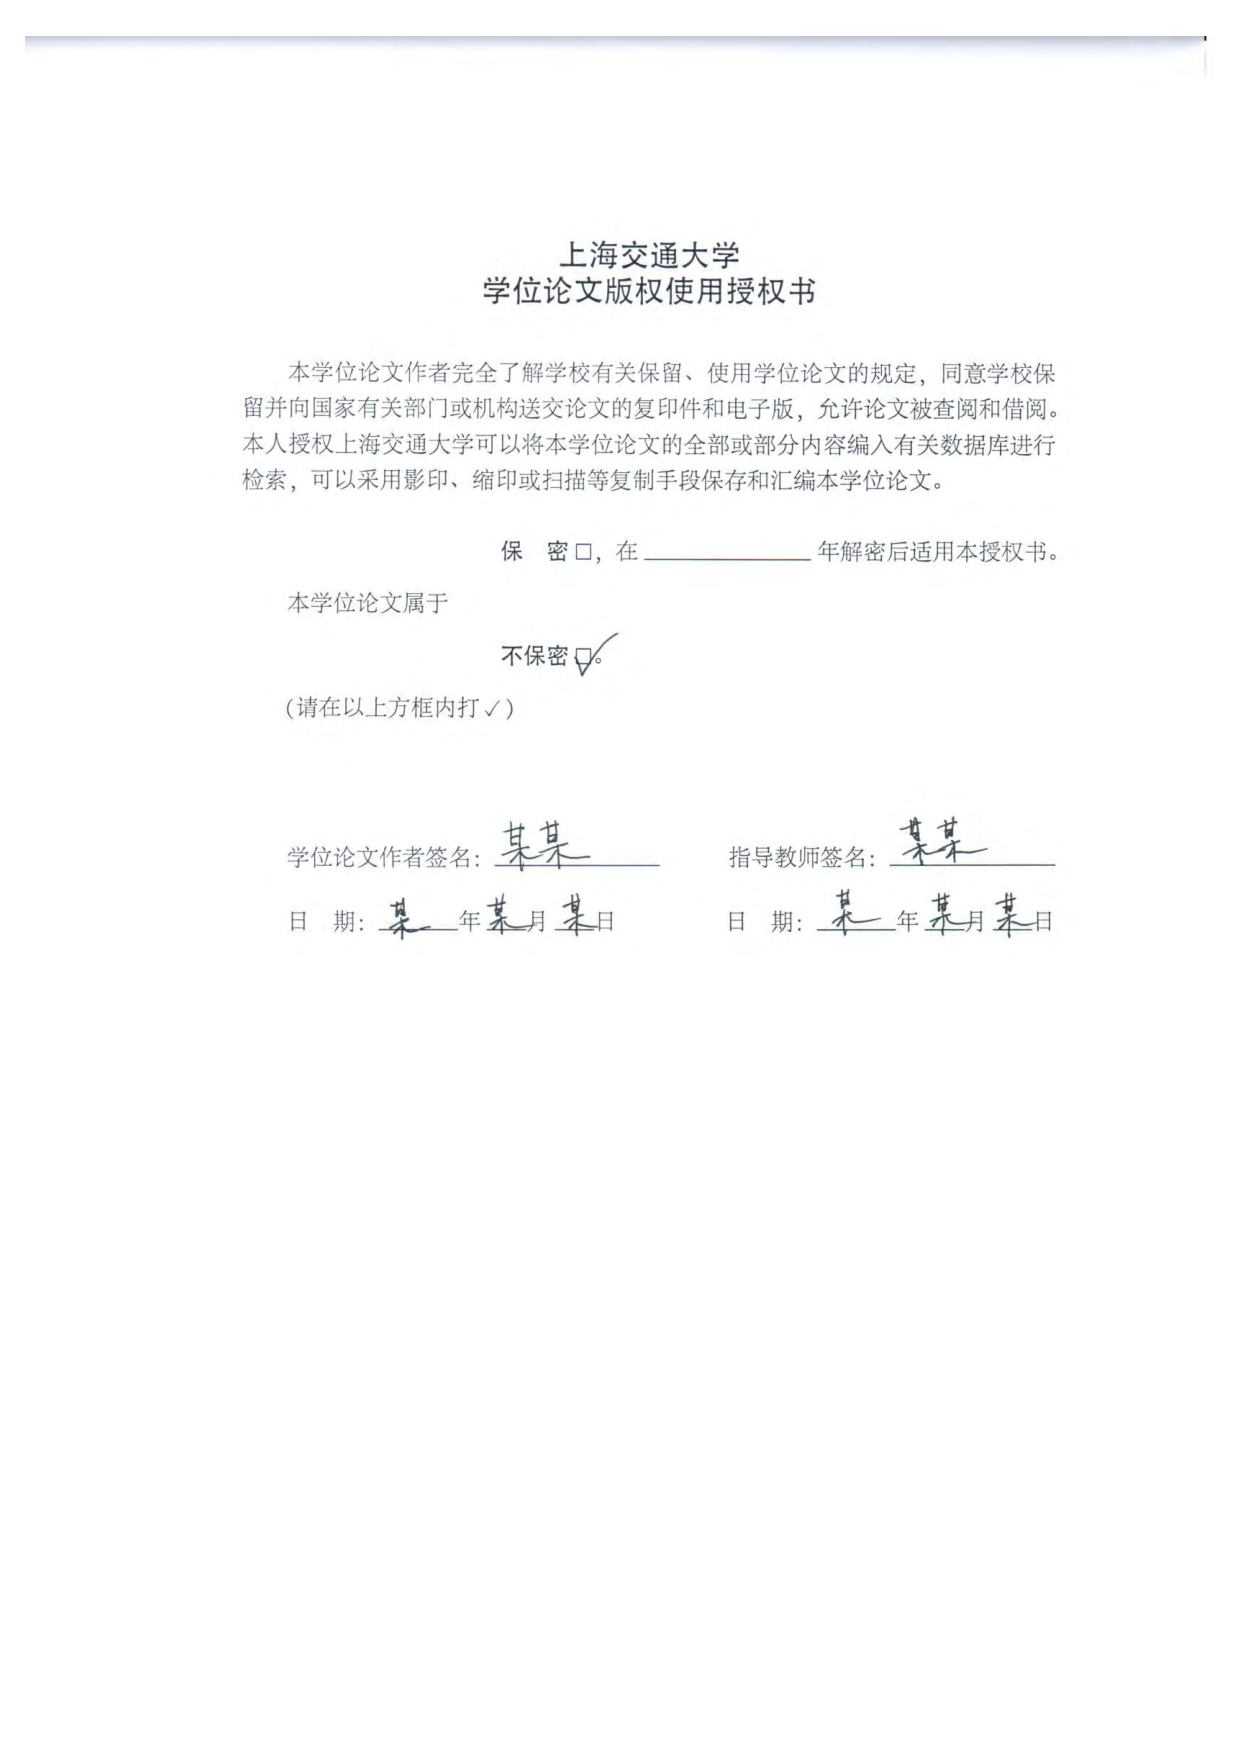
\includepdf{pdf/authorization.pdf}
	\cleardoublepage
\else
	\makeDeclareOriginal
	\makeDeclareAuthorization
\fi
\makeatother


\frontmatter 	% 使用罗马数字对前言编号

%% 摘要
\pagestyle{main}
%# -*- coding: utf-8-unix -*-
%%==================================================
%% abstract.tex for SJTU Master Thesis
%%==================================================

\begin{abstract}

\keywords{\large 低阶模型生成 \quad 拓扑简化 \quad 双图决策树}
\end{abstract}

\begin{englishabstract}

\englishkeywords{\large Low-order model generation, topological simplification, Graph-Pair Decision Diagram (GPDD)}
\end{englishabstract}



%% 目录、插图目录、表格目录
\tableofcontents
\listoffigures
\addcontentsline{toc}{chapter}{\listfigurename} %将插图目录加入全文目录
\listoftables
\addcontentsline{toc}{chapter}{\listtablename}  %将表格目录加入全文目录
% \listofalgorithms
% \addcontentsline{toc}{chapter}{代码索引}  %将表格目录加入全文目录

% %# -*- coding: utf-8-unix -*-
\chapter{主要符号对照表}
\label{chap:symb}

\begin{longtable}{rl}
$\epsilon$     & 介电常数 \\
 $\mu$ 		& 磁导率 \\
 $\epsilon$     & 介电常数 \\
 $\mu$ 		& 磁导率 \\
 $\epsilon$     & 介电常数 \\
 $\mu$ 		& 磁导率 \\
 $\epsilon$ 	& 介电常数 \\
 $\mu$ 		& 磁导率 \\
 $\epsilon$     & 介电常数 \\
 $\mu$ 		& 磁导率 \\
 $\epsilon$     & 介电常数 \\
 $\mu$ 		& 磁导率 \\
 $\epsilon$     & 介电常数 \\
 $\mu$ 		& 磁导率 \\
 $\epsilon$ 	& 介电常数 \\
 $\mu$ 		& 磁导率 \\
 $\epsilon$     & 介电常数 \\
 $\mu$ 		& 磁导率 \\
 $\epsilon$     & 介电常数 \\
 $\mu$ 		& 磁导率 \\
 $\epsilon$     & 介电常数 \\
 $\mu$ 		& 磁导率 \\
 $\epsilon$ 	& 介电常数 \\
 $\mu$ 		& 磁导率 \\
 $\epsilon$     & 介电常数 \\
 $\mu$ 		& 磁导率 \\
 $\epsilon$     & 介电常数 \\
 $\mu$ 		& 磁导率 \\
 $\epsilon$     & 介电常数 \\
 $\mu$ 		& 磁导率 \\
 $\epsilon$ 	& 介电常数 \\
 $\mu$ 		& 磁导率 \\
 $\epsilon$     & 介电常数 \\
 $\mu$ 		& 磁导率 \\
 $\epsilon$     & 介电常数 \\
 $\mu$ 		& 磁导率 \\
 $\epsilon$     & 介电常数 \\
 $\mu$ 		& 磁导率 \\
 $\epsilon$ 	& 介电常数 \\
 $\mu$ 		& 磁导率 \\
 $\epsilon$     & 介电常数 \\
 $\mu$ 		& 磁导率 \\
 $\epsilon$     & 介电常数 \\
 $\mu$ 		& 磁导率 \\
 $\epsilon$     & 介电常数 \\
 $\mu$ 		& 磁导率 \\
 $\epsilon$ 	& 介电常数 \\
 $\mu$ 		& 磁导率 \\
 $\epsilon$     & 介电常数 \\
 $\mu$ 		& 磁导率 \\
 $\epsilon$     & 介电常数 \\
 $\mu$ 		& 磁导率 \\
 $\epsilon$     & 介电常数 \\
 $\mu$ 		& 磁导率 \\
\end{longtable}
 % 主要符号、缩略词对照表

\mainmatter	% 使用阿拉伯数字对正文编号

%% 正文内容
\pagestyle{main}
%# -*- coding: utf-8-unix -*-
%%==================================================
%% chapter01.tex for SJTU Master Thesis
%%==================================================

\chapter{绪论}
\label{chap:intro}

本章首先介绍模拟集成电路设计的概况,指出其设计过程中由于计算机辅助设计的缺失带来的设计效率低下的问题。
进而回顾符号化分析方法在这一问题上所作出的诸多努力,并简要介绍并比较相应成果。
最后介绍本文的主要内容,并给出文章组织安排。

\section{模拟集成电路设计方法概述}
\label{sec:intro:analog}
随着半导体产业的不断发展与电子设备的不断的推陈出新,对集成电路设计的时效性及高效性提出了更高的要求。
同时,越来越多的功能被集成在同一块芯片内部,从而推动了SoC(System-on-Chip)概念的形成,对电路设计带来更多困难与挑战\parencite{Saleh-SoC-2006}。
作为集成电路设计的两大重要分支,数字集成电路设计和模拟集成电路设计的设计方法决定了SoC设计效率,同时保证了电路性能与可靠性。
其中,由于电子设计自动化(Electronic Design Automation, EDA)工具的成熟,数字集成电路设计的效率已远远超过模拟电路设计\parencite{Ghasi-VLSID-2009}。
数字电路在整个设计流程,如电路综合、验证、自动布局布线等,均有对应的EDA工具做相应的支持。
除此之外,数字集成电路中由于有IP(Intellectual Property)核的支持,可以轻松地对功能模块进行重用,大大方便了数字电路工程师进行电路设计。
然而相对应的,模拟电路由于其电路性能特征描述的困难以及针对不同应用设计变化复杂等原因一直导致其IP化进程并不十分顺利\parencite{Zheying-ICASIC-2003, Saleh-SoC-2006}。

\begin{figure}[!htp]
	\centering
	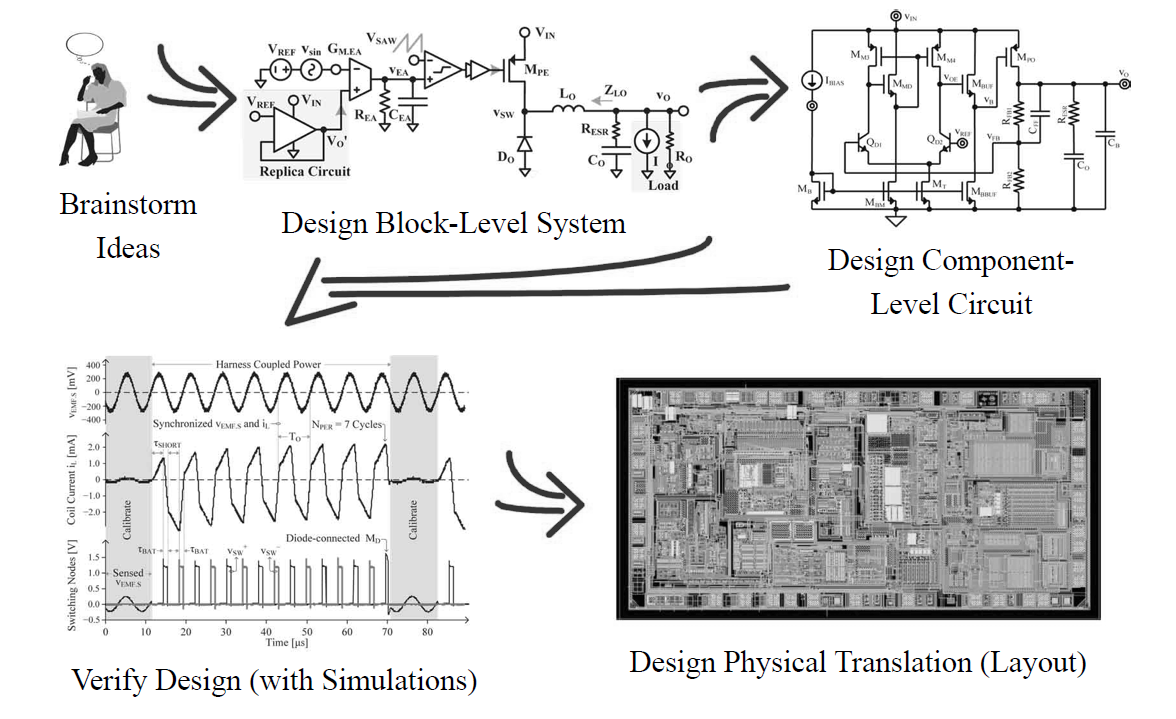
\includegraphics[width=0.9\textwidth]{chap1/AICWhy.png}
	\bicaption[fig:AICWhy]{基本模拟集成电路设计流程}{基本模拟集成电路设计流程\parencite{Gabriel-AICWhy}}{Fig}{Basic analog integrated circuits design procedure \parencite{Gabriel-AICWhy}}
\end{figure}

模拟集成电路在现代SoC设计中基本只占这个芯片面积的10\%-50\%,然而这个设计流程中有近50\%-90\%的时间用于模拟部分的设计与测试\parencite{Gabriel-AICWhy}。
而且往往由于模拟电路的设计错误,可能导致多次流片验证,增加了设计成本。
模拟集成电路自与1964年诞生以来\parencite{Thomas-AICHistory-2007},基本一直遵循图\ref{fig:AICWhy}中的设计流程。
电路设计往往从整体系统建模开始,然后根据系统的整体性能指标,给出更具体的电路功能模块的性能指标。
然后,参照模块性能,选择合适的电路结构,并结合电路仿真结果,确定元件参数。
综合所有功能模块,在完成系统层面仿真。
最后,手工绘制版图后,并检查无误后,送至工艺厂进行生产。
由于上述设计流程限制,模拟电路设计往往受到以下条件制约:

\begin{enumerate}[label=\emph{\alph*})]
	\item 上述大部分流程均为人工计算设计得到,缺乏计算机辅助设计流程,大部分情况下需要工程师的个人经验作为设计依据。
	\item 上述流程往往需要多次反复,根据仿真结果一再调整结果,带来设计效率的低下。
	\item 模拟电路仿真往往花费大量时间,特别是在系统级的仿真中,任何参数的调整带来巨大的时间损耗,拉长了整个设计周期。
\end{enumerate}

可以看到,上述原因主要是由于模拟电路设计缺乏计算机辅助设计工具,导致设计方法因人而异,没有形成系统化的设计体系所造成的。
其中,模拟电路的建模是关键的一环。
如果存在系统化自动化的模拟电路建模方法,那么首先由于模型的建立方式的统一,会带来设计人员学习理解的方便。
同时,由于所建立的电路模型中可以带有电路元件参数,直接将电路性能与电路元件取值联系在一起,方便了电路设计的优化流程。
另外,自动化建模可以在系统仿真层面大大加快设计效率,提升仿真速度。
故可以看到提出行之有效的系统化自动化模拟电路建模方案将在一定程度上有效地解决上述三个制约条件,对加快电路设计效率有着至关重要的作用。

\section{符号化分析方法}
\label{sec:intro:symbolic}

目前,模拟电路仿真主要采用以SPICE为基础的数值化仿真工具\parencite{Nagel-SPICE-1973},如Cadence公司的Spectre以及Synopsys的HSPICE仿真器等。
数值仿真器以其稳定高效的数值求解结果成为业界的常用仿真工具。
然而数值仿真方法最大的问题在于其仿真结果与电路元件参数的取值脱节,很难从电路的仿真结果对电路元件的取值反推相应的结果。
这导致电路工程师,特别是经验不丰富的工程师,在不确定电路元件与性能关系的情况下,只能对电路元件取值进行盲目的调整,以期达到所要求的性能指标。
为了克服这一困难,本文采用符号化仿真方法对电路进行分析。

\subsection{符号化分析方法回顾}
\label{subsec:intro:symbolic:review}

上世纪90年代,另一种电路仿真方法符号化仿真方法得到了许多关注\parencite{Lin-Symb}。
与数值化仿真不同,符号化仿真方法会直接建立小信号电路传输函数与电路元件之间的表达式,然后通过所求的电路传输函数表达式进行求解,如图\ref{fig:symbolic}所示的流程。

\begin{figure}[!htp]
	\centering
	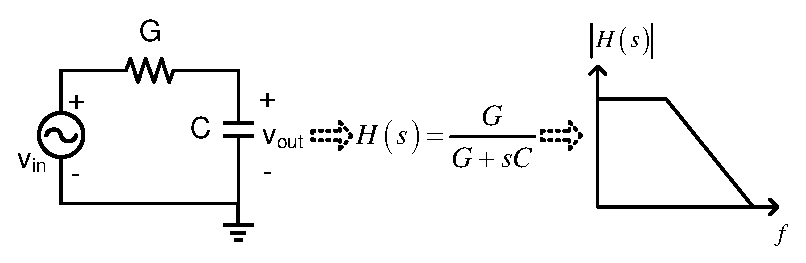
\includegraphics[width=0.7\textwidth]{chap1/symbolic.eps}
	\bicaption[fig:symbolic]{符号化分析流程}{符号化分析流程}{Fig}{General symbolic analysis procedure}
\end{figure}

这种电路分析方式带来诸多数值化仿真不能得到的好处,主要可以归纳为以下几点:

\begin{enumerate}[label=\emph{\alph*})]
	\item 可以直观地通过符号化公式告知电路设计者所有电路元件参数对电路的作用,有助于工程师进行优化调整及相应的分析。
	\item 在构造解析表达式后,在电路元件重新调整后,可以直接通过得到的公式进行仿真求解,避免费时的数值矩阵迭代过程。
	\item 可以通过求解得到的公式对电路进行表征,构建相应的电路模型,用于将来的模拟电路功能模块综合、验证等功能的实现。
\end{enumerate}

构建符号化表达式十分多样,过去开发了多种不同的符号化求解方式,如矩阵行列式展开求解\parencite{Gielen-ISAAC-1989}、利用Mason规则求解信号流图\parencite{Nebel-SFG-1995,Fino-SFG-1998}、双图枚举\parencite{Shieu-TG-1974}等。
这些算法都可以求解一个线性电路的传输函数;针对如含有MOSFET的非线性电路,求解器则会通过静态工作点仿真得到非线性元件的小信号模型,并带入计算。

然而,由于符号化分析方法本身性质决定,随着电路规模的增长,符号化分析中符号化项的规模也呈指数级增长,\parencite{Gielen-SymbSurvey-1998}对各种不同的符号化方法中的规模增长进行了验证与比较。
这在很大程度上限制了符号化方法在大规模电路中的应用,甚至当时提出的多数算法难以对一个完整的运放电路进行符号化分析。
其次多数符号化方法,与节点分析法、回路分析法等传统电路分析方法差异比较大,很多算法都存在规则繁琐,不利于手工计算的问题,所以相对其推广也更加不如数值化分析方法。

\subsection{双图决策树(GPDD)符号化分析方法}
\label{subsec:intro:symbolic:gpdd}

为解决符号化表达式增长过快的问题,Sheldon X.-D. Tan于2000年附近提出了DDD(Determinant Decision Diagram)符号化方法。
他们使用Cramer法则计算电路传输函数,并利用二分决策图(Binary Decision Diagram, BDD)结构\parencite{Bryant-BDD-1986}来存储计算过程中得到的符号化表达式\parencite{Sheldon-DDD-2000}。
这种方法有效地缓解了符号化公式占用大量存储空间的问题,但是其所保存的符号化公式存在非常多的对消项。(对消项会在第\ref{chap:simp}章有更详细的描述。)
这造成了计算机计算过程中的数值误差的累积,其求解结果有一定误差。

2006年附近,G. Shi等人提出了双图决策树(Graph-Pair Decision Diagram, GPDD)方法\parencite{ChenWeiWei-Thesis,GShi-GPDD-2013,GShi-GPDD,GShi-GPDDSurvey-2013}。
此方法也利用了BDD结构,对符号化项进行隐式枚举,从而保证了与DDD相当的高效的空间利用率。
虽然,这种方法的符号化结果规模仍然随着电路规模呈指数级增长,但是由于相较早期的符号化方法,其增长速度较慢,以足以分析一个运放这样规模的电路。
同时,该方法从理论保证了对消项不会在最终得到的符号化表达式中出现,从而可以得到非常精确的计算结果。

近几年来,GPDD方法从软件实现仿真到电路建模优化等多方面得到了许多发展。
\parencite{XuHui-Hier-2011, LiXiaopeng-Hier-2011, SongYang-Hier-2012}中使用了层次化的方法,从而实现了对较大规模模拟集成电路的分析;
\parencite{MengXiaoxuan-Sens-2009,WengBinbin-Sens-2011,ChenJiajun-Sens-2012}中利用符号化敏感度分析方法,对电路元件敏感性进行了探索,并开发了自动调整运放尺寸的算法;
\parencite{ZhangHe-Slew-2011,ZhangAilin-Slew-2015}通过Moment Matching的方法对电路零极点进行建模,从而得到运放时域电路模型;
\parencite{ChengJiandong-SC-2013}实现了对开关电容电路的仿真,从而得到了z域的GPDD仿真方法;
\parencite{ChengJiandong-SDM-ASPDAC-2013, ChengJiandong-SDM-TENCON-2013}进一步将其应用到Sigma-Delta调制器中。

下面通过一例子对这种方法进行详细介绍。

\begin{exmp}
RC电路的GPDD构造示例
	
考虑如图\ref{fig:RC_cir}所示的RC低通滤波器电路,这里希望求取电路的从输入电压至电容两端输出电压的传输函数。
根据电路结构,构造如图中右侧所示的图,将电路元件抽象为图中的边,用电路元件的导纳值作为元件的符号。
其中电路的输入输出关系,我们用从输出控制输入的受控源$X$来进行标识,并作为GPDD结构的根节点。
这里由于是输出电压控制输入电压,故为电压控制电压源(VCVS),在图中即为对应的紫色VC和VS边。
	
\begin{figure}[!htp]
	\centering
	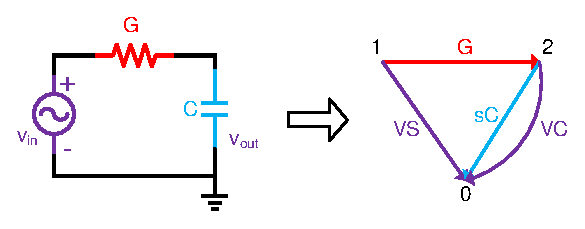
\includegraphics[width=0.6\textwidth]{chap1/RC_cir.eps}
	\bicaption[fig:RC_cir]{RC低通滤波电路及对应原始图}{RC低通滤波电路及对应原始图}{Fig}{RC low-pass filter \& its corresponding graph}
\end{figure}

根据双图电路分析理论\parencite{Lin-Symb},可以知道在上述电路中可被接受的生成树对仅有图\ref{fig:RC_tree}中所示的三对,同时每一个生成树对构成了一个符号化的项。
如将这些项相加,并使它等于0,则可求得电路的传输函数:

\begin{equation}
\label{eq:RC}
- XG + G + sC = 0 \Rightarrow H\left( s \right) = \frac{1}{X} = \frac{G}{G + sC}
\end{equation}

\begin{figure}[!btp]
	\centering
	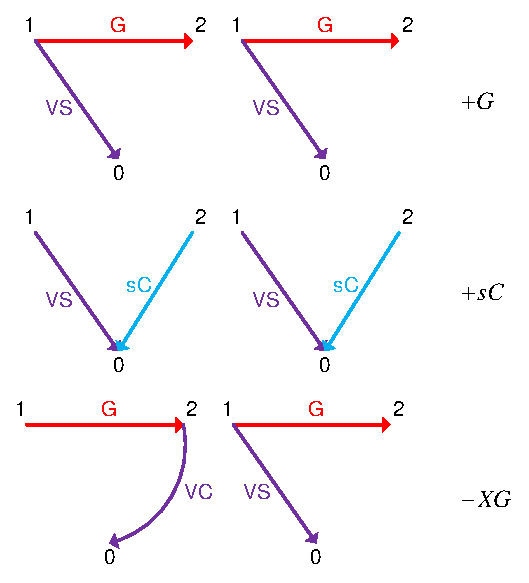
\includegraphics[width=0.55\textwidth]{chap1/RC_tree.eps}
	\bicaption[fig:RC_tree]{RC低通滤波电路生成树对}{RC低通滤波电路生成树对}{Fig}{Spanning tree pairs in RC low-pass filter}
\end{figure}

为了能够快速枚举原始图中所有的符合条件的生成树对,GPDD算法是用了类似图\ref{fig:RC_GPDD}所示的BDD结构来保存枚举结构\parencite{GShi-GPDD-2013}。
GPDD结构每一层有且仅有一个元件符号,每个GPDD节点有两个2儿子,左儿子用实线与下面的节点连接,右儿子用虚线与下面的节点连接。
不同节点可以共享同一个儿子,这也是GPDD之所以可以用较少空间存储大量符号化项的原因,类似于多项式的公因式提取。
所有的节点必然终结于$1$结点或$0$结点。
可以看到这个GPDD结构中共有3条从根节点通往$1$结点的路径,如路径经过了实线,那么实线出发点的符号会出现在该符号项中;如是虚线,则不出现。
经验证,可知道这3条路径正是指代前面的3个生成树对,从而可以保存了电路的传输函数的符号化表达。

\begin{figure}[!htp]
	\centering
	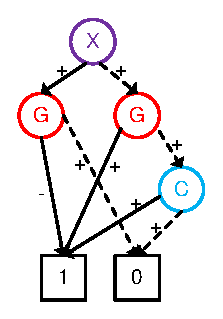
\includegraphics[width=0.2\textwidth]{chap1/RC_GPDD.eps}
	\bicaption[fig:RC_GPDD]{RC电路的GPDD结构示例}{RC电路的GPDD结构示例}{Fig}{GPDD structure of RC circuit}
\end{figure}

\begin{figure}[!htp]
	\centering
	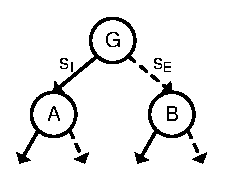
\includegraphics[width=0.25\textwidth]{chap1/evalGPDD.eps}
	\bicaption[fig:evalGPDD]{GPDD求值规则}{GPDD求值规则}{Fig}{The evaluation rule for GPDD}
\end{figure}

这里简要介绍GPDD结构的计算方法。如图\ref{fig:evalGPDD}所示,对于GPDD结构中某个节点$G$的求值,用$f_{G} \left( G \right)$来标示。
在递归得求得其左右子GPDD结构的值后,用其符号本身$G$乘以以实现相连的$A$节点的值$f_{A} \left( A \right)$,并加上虚线相连的$B$节点的值$f_{B} \left( B \right)$。
注意这里,需记得考虑实线及虚线上所标识的符号$s_I$和$s_E$,$s_I$和$s_E$仅为正负关系。总结可如下式所示:

\begin{equation}
\label{eq:evalGPDD}
f_{G} \left( G \right) = s_I G f_{A} \left( A \right) + s_E f_{B} \left( B \right)
\end{equation}

如使用式\ref{eq:evalGPDD}可以验证得到式\ref{eq:RC}的结果。
根据该计算规则,可以通过自底向上遍历整个GPDD结构,求得电路传输函数。
在根节点处,无需显式求解令方程等于0的传输函数值。
假设根节点$X$左儿子为$N$,符号为$s_N$;右儿子为$D$,符号为$s_D$。那么电路传输函数即为:

\begin{equation}
\label{eq:evalGPDDRoot}
s_N  X f_N\left(N\right) + s_D f_D\left(D\right) = 0 \Rightarrow H \left( s \right) = \frac{1}{X}= - s_N s_D \frac{f_N\left(N\right)}{f_D\left(D\right)}
\end{equation}

\end{exmp}

\section{电路模型符号化简化方法简介}
\label{sec:intro:simp}

另一方面由于符号化的

\subsection{构建前简化方法}
\label{subsec:intro:simp:SBG}
\parencite{Hsu-SBG-1994}
\subsection{构建中简化方法}
\label{subsec:intro:simp:SDG}
\parencite{Fern-SDG-1994}
\subsection{构建后简化方法}
\label{subsec:intro:simp:SAG}
\parencite{Zivkovic-TopoSimp-1995,Sheldon-DDDSimp-1999}

\subsection{符号化模型降阶}
\label{subsec:intro:symbolic:smor}
\parencite{GShi-SMOR-2006}

\section{主要贡献与章节安排}

\label{sec:intro:org}
%# -*- coding: utf-8-unix -*-
%%==================================================
%% chapter02.tex for SJTU Master Thesis
%% Encoding: UTF-8
%%==================================================

\chapter{电路拓扑符号化自动降阶模型生成方法}
\label{chap:simp}

上一章介绍了电路模型对电路设计的重要性,可见电路低阶模型本身的提出也应有一定方法可以指导其生成。
只有在拥有可靠的模拟集成电路低阶模型的情况下,电路设计工程师才有可能对电路做出进一步的理论分析,从而指导进一步的设计。
本章给出了本文最关键的算法:采用拓扑简化方法得到的低阶模型自动生成算法,并给出了其相关的测试结果,佐证了算法的有效性。

\section{双图决策树符号约简}
\label{sec:simp:GPDD}

\subsection{电路元件极值与元件拓扑的关系}
\label{subsec:simp:GPDD:TopoLimit}

本课题采用拓扑简化的方法实现电路模型的自动生成。
所以电路元件的拓扑结构对于分析本身有非常重要的作用。
我们发现电路的元件的极限取值可以代表新的简化的电路拓扑结构。
这正可以成为我们对电路简化的基石。
当我们考虑需要将一个电路中的元件删去时,即可认为是电路这个元件选取了极限的取值导致。
当然一个电路元件删去过程中,往往存在两个电路元件删去方式:短路和断路。

\begin{figure}[!htp]
	\centering
	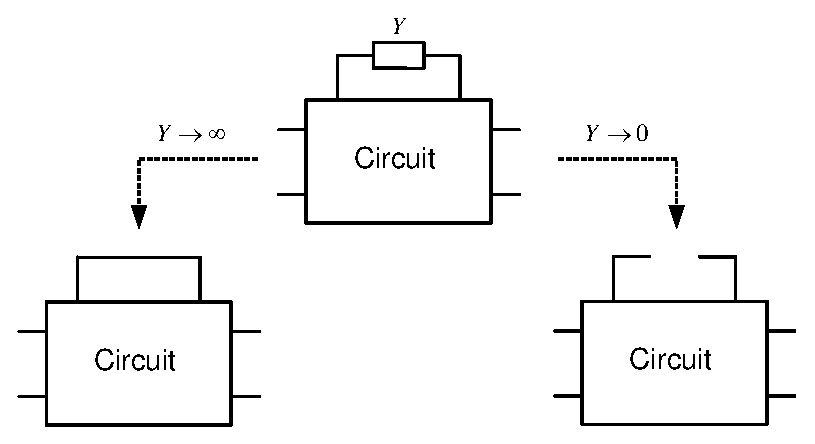
\includegraphics[width=0.7\textwidth]{chap2/LimitTopo.eps}
	\bicaption[fig:limittopo]{导纳在极限取值情况下的拓扑结构改变}{导纳在极限取值情况下的拓扑结构改变}{Fig}{Topological adjustment of impedance whose value changes to limit value}
\end{figure}

如图\ref{fig:limittopo}所示,假设在一个电路中有一处导纳值为$Y$的阻抗。
现在我们用两个极限的值$\infty$和$0$去替代这个导纳值$Y$。
可以看到当,导纳值$Y$趋向于无穷大时,由于此时其相应的阻抗$Z$为零,所以此时这个阻抗变为短路的电路结构;
然而当导纳值$Y$趋向于零时,由于此时其阻抗值$Z$为无穷大,这种情况下电路结构变为阻抗两端的两个节点变为了断路的状态。
可以看到,这样我们就可以用电路元件的极限取值来替代线性阻抗元件(R/L/C)的拓扑变化。

然而,在小信号电路中,我们知道不仅存在线性阻抗元件(R/L/C),另外还有四种受控信号源,分别为:电压控制电压源(VCVS),电流控制电流源(CCCS),电压控制电流源(VCCS),电流控制电压源(CCVS)。
我们发现在以上两种极限取值仍然适用于这四种受控源,特别是在取无穷大情况下,它们都会成为一种称为Nullor的电路元件,如图\ref{fig:nullor}。

\begin{figure}[!htp]
	\centering
	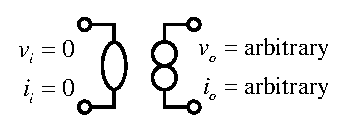
\includegraphics[width=0.35\textwidth]{chap2/SymbolNullor.eps}
	\bicaption[fig:nullor]{Nullor元件符号}{Nullor元件符号}{Fig}{Nullor symbol}
\end{figure}

可以看到,Nullor元件假设其输入端的输入电流和电压均为0,有着任意大小的输出能力。
Nullor这种元件与传统的模拟电路学习中接入负反馈中的理想运算放大器的虚短虚断的性质是一致。
但由于Nullor本身往往可以与电路中别的元件合并,并且不会出现在电路最后的模型中,这一点会在本章中节\ref{subsubsec:simp:res:cir:fd}中看到。

\begin{table}[!htbp]
	\bicaption[tab:symbollimit]{电路元件极限取值的拓扑结构}{电路元件极限取值的拓扑结构}{Table}{Circuit element topology whose value is infinity or zero}
	\centering
	\begin{tabular}{c|c|c}
		\hline
		\multirow{2}{*}{Symbol} & \multicolumn{2}{c}{Value}\\
		\cline{2-3} 
		& $\infty$ & $0$\\
		\hline
		\parbox[c]{0.11\textwidth}{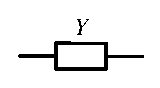
\includegraphics[width=0.11\textwidth]{chap2/Impedance.eps}} & 
		\parbox[c]{0.11\textwidth}{
\includegraphics[width=0.11\textwidth]{chap2/Impedance-Short.eps}} & 
		\parbox[c]{0.11\textwidth}{
\includegraphics[width=0.11\textwidth]{chap2/Impedance-Open.eps}} \\
		\hline
		\parbox[c]{0.2\textwidth}{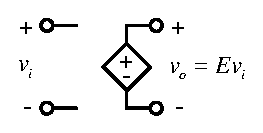
\includegraphics[width=0.2\textwidth]{chap2/VCVS.eps}} & 
		\parbox[c]{0.11\textwidth}{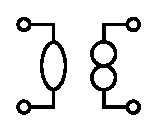
\includegraphics[width=0.11\textwidth]{chap2/Nullor.eps}} & 
		\parbox[c]{0.11\textwidth}{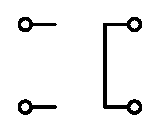
\includegraphics[width=0.11\textwidth]{chap2/VCVS-Open.eps}} \\
		\hline
		\parbox[c]{0.2\textwidth}{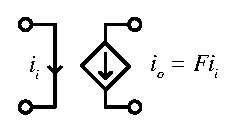
\includegraphics[width=0.2\textwidth]{chap2/CCCS.eps}} & 
		\parbox[c]{0.11\textwidth}{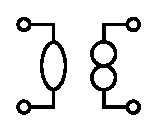
\includegraphics[width=0.11\textwidth]{chap2/Nullor.eps}} & 
		\parbox[c]{0.11\textwidth}{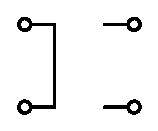
\includegraphics[width=0.11\textwidth]{chap2/CCCS-Open.eps}} \\
		\hline
		\parbox[c]{0.2\textwidth}{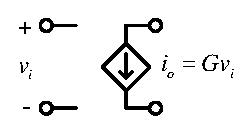
\includegraphics[width=0.2\textwidth]{chap2/VCCS.eps}} & 
		\parbox[c]{0.11\textwidth}{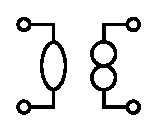
\includegraphics[width=0.11\textwidth]{chap2/Nullor.eps}} & 
		\parbox[c]{0.11\textwidth}{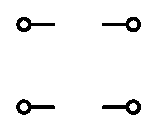
\includegraphics[width=0.11\textwidth]{chap2/VCCS-Open.eps}} \\
		\hline
		\parbox[c]{0.2\textwidth}{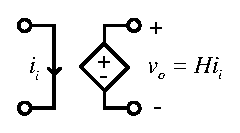
\includegraphics[width=0.2\textwidth]{chap2/CCVS.eps}} & 
		\parbox[c]{0.11\textwidth}{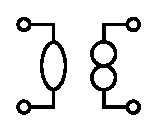
\includegraphics[width=0.11\textwidth]{chap2/Nullor.eps}} & 
		\parbox[c]{0.11\textwidth}{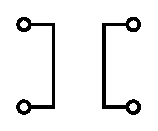
\includegraphics[width=0.11\textwidth]{chap2/CCVS-Open.eps}} \\
		\hline
	\end{tabular}
\end{table}

为了说明受控源取极限值情况下电路拓扑结构的变化,这里仅以VCVS为例进行说明。
所有小信号分析中用到的阻抗和四种受控源的拓扑变化可以参考表\ref{tab:symbollimit}。
我们知道VCVS的输入输出电压关系如下式所示:

\begin{equation}
	v_o = E v_i
\end{equation}

这里,$v_i$和$v_o$分别为VCVS的输入输出电压,$E$则为VCVS的放大倍数。
首先我们考虑$E$取无穷大的情况,为了电路仍然能正常工作,我们知道输出电压$v_o$应为有限值,而其中$E$为无穷大,那么根据基本微积分的知识,我们知道此等式中的输入电压$v_i$为零。
另外由于VCVS的输入端测量电压,所以本来就限定输入的电流$i_i$为零,所以其形成了Nullor的虚短虚断的性质。
另外当$E$的取值为零时,根据VCVS本身的关系,即可得出输出端电压为零,所以输出端两端电压一致,即此端口可用一根导线连接起来,加之本为断路连接的输入端,故VCVS可约减为表\ref{tab:symbollimit}中的结构。

\subsection{双图决策树和电路拓扑的关系}
\label{subsec:simp:GPDD:TopoGPDD}

上一小节已经将电路的极限取值与电路的拓扑结构变化建立起了联系,而此时电路元件的极限求值成为了新的问题。
由于在整个算法过程中,需要多次计算不同拓扑结构下电路性能表现,这要求了高效的计算方法的支持。
然而GPDD结构本身蕴含了对电路拓扑结构,可以轻松方便地在其中对不同的电路拓扑结构求值,这支持了下一节所介绍的简化算法。

\begin{figure}[!htp]
	\centering
	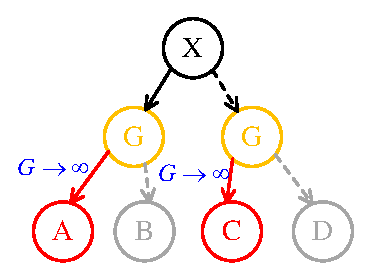
\includegraphics[width=0.35\textwidth]{chap2/GPDDTopo.eps}
	\bicaption[fig:GPDDTopo]{符号极限取值情况下GPDD的计算方法}{符号极限取值情况下GPDD的计算方法}{Fig}{Calculation rule for GPDD under limit value}
\end{figure}

我们知道根据电路基本原理,并且结合GPDD的计算规则,针对类似图\ref{fig:GPDDTopo}这样的GPDD结构,我们可以求得类似下式的电路传输函数表达式(为了说明的方便,这里忽略了GPDD中连接节点的边上的符号):

\begin{equation}
H \left( s \right) = \frac{{{f_A}\left( A \right)G + {f_B}\left( B \right)}}{{{f_C}\left( C \right)G + {f_D}\left( D \right)}}
\end{equation}

考虑目前我们需要对电路中的元件$G$求取极限值,并计算新的符号化传输函数公式。
这里假设元件$G$位于GPDD符号表中的第一层,这里层数不影响极限取值的计算,只是为方便说明特意假设。
我们可以得到在$G$元件取无穷大情况下,电路的新传输函数为:

\begin{equation}
\label{eq:simpGPDD}
\mathop {\lim }\limits_{G \to \infty } H \left( s \right) = \frac{{f_A}\left( A \right)}{{f_C}\left( C \right)}
\end{equation}

首先,十分显然地,可以看到取极限后首先原有的符号$G$从公式消失了,这也暗示了电路拓扑的简化,即$G$从电路中以短路的方式被删去了。
另外,可以发现,在式\ref{eq:simpGPDD}中所有的保留下的符号项均是在GPDD结构中以红色实线相连的红色节点$A$和$C$的值。
由于,我们知道,GPDD结构中实线相连的节点均采用乘法进行计算,故在求取极限的过程中,其相应的系数得到保留。
故当某一符号元件需取无穷大情况下的值时,在GPDD计算过程中,仅需计算GPDD对应符号所有节点左儿子的值即可,所有的右儿子忽略。
同样的,我们知道当对一个电路元件取值零时,GPDD计算中仅需考虑该元件所有节点右儿子的值即可,左儿子的值则忽略,而且算法设计简单,仅需直接用0带入符号值即可。
总结来说,GPDD中某个节点左儿子承担了该节点符号取值无穷大情况(阻抗短路,受控源Nullor)下的电路性能,而右儿子为该节点符号取值零情况(阻抗断路,受控源删去)下的电路性能,当符号本身有一定值时,则为两者的折衷。

当然需要注意的是,在求某一个符号为无穷大时,由于特殊的GPDD规模缩小的算法,类似Reduction、Zero-Suppression等算法\parencite{GShi-GPDD-2013,GShi-GPDD},可能存在有排序在$G$之上的符号直接与排序在$G$之下的符号节点相连的情况。
这种情况需特别注意,因为这种项中不包含$G$符号,故取极限值时,并非系数,也需忽略。
具体的GPDD中符号约减下的计算方法已在\parencite{HanbinHu-Thesis}有阐释,这里不再赘述。

下面通过一个例子展示电路拓扑结构变化对GPDD结构的影响,以直观了解这两者之间的关系。

\begin{exmp}
RLC电路向RC电路简化过程中GPDD结构比较

图\ref{fig:RLC}中展示了一个RLC串联的简易电路,与之前给出的图\ref{fig:RC_cir}相比较,这里多出了电感元件。
可以看到如果这个电感$L$如果取值为零,那么其导纳$Y=\left(s L\right)^{-1}$,即导纳为无穷大情况,即可得到RC电路的电路图。

\begin{figure}[!htp]
	\centering
	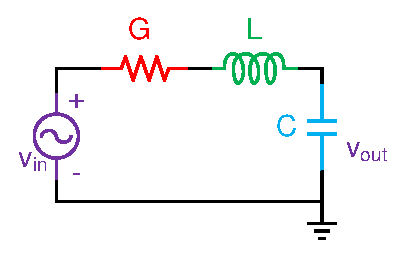
\includegraphics[width=0.4\textwidth]{chap2/RLC.eps}
	\bicaption[fig:RLC]{RLC电路示意图}{RLC电路示意图}{Fig}{RLC circuit example}
\end{figure}

此RLC电路对应的GPDD结构展示在图\ref{fig:RLCvsRC}中的左侧。这张图右侧是展示的RC电路对应的GPDD结构。
可以看到通过两侧曲线包围起来的结构是一致的,而且均与电感符号$L$的左儿子相连,这与之前的论述是相符的。
同时可以看到,由于RC的GPDD结构蕴含在RLC的GPDD结构中,故可以直接在RLC的GPDD结构上对RC电路的GPDD进行求值。
这表示了GPDD拥有在同一个BDD数据结构中求解多种不同电路拓扑的能力,这大大方便了符号简化电路自动生成算法的设计。
这种能在同一个符号化结构中表达不同拓扑结构电路的能力是别的符号化方法不具备的,也是GPDD相比其他的符号化方法一大优势所在。

\begin{figure}[!htp]
	\centering
	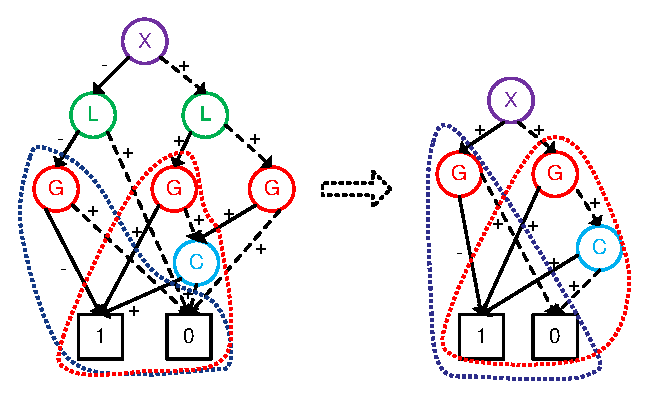
\includegraphics[width=0.7\textwidth]{chap2/RLCvsRC.eps}
	\bicaption[fig:RLCvsRC]{符号极限取值情况下GPDD结构示例}{符号极限取值情况下GPDD结构示例}{Fig}{GPDD structure example under limit value}
\end{figure}

\end{exmp}

GPDD对降阶模型的求解的优势在于在一次符号表达构造的情况下,可以在多次同一个结构中求得对应与不同简化模型的电路传输函数。
符号化构造往往大量计算时间花费在符号化表达式的构造上,而其求值往往是高效的稳定的。
故可以如将构造的时间平摊在之后的多次求值上,仍然得到了许多计算上的便利。
同时,如采用传统的数值化求解器,需要对电路矩阵做行列合并等操作,操作复杂。

\section{符号化降阶模型生成算法与流程}
\label{sec:simp:alg}

在建立电路拓扑与元件取值之间的关系,并使用GPDD这个便利的工具可方便求取电路拓扑变化情况下的电路性能的条件下,本节对符号化降阶模型生成算法进行全面的介绍。
首先,将介绍算法的总体流程,并逐一介绍其中每个流程具体细节,并给出简化过程中一些特殊情况的处理。
本文讨论中,我们主要针对运算放大器的设计进行讨论,故我们接下来的讨论将均针对运算放大器设计。

\subsection{简化算法总体流程}
\label{subsec:simp:alg:top}

降阶模型的建立,我们将其看作一个电路拓扑元件简化的过程,总的流程可参见图\ref{fig:SimpProcedure}的流程示意。

\begin{figure}[!htp]
	\centering
	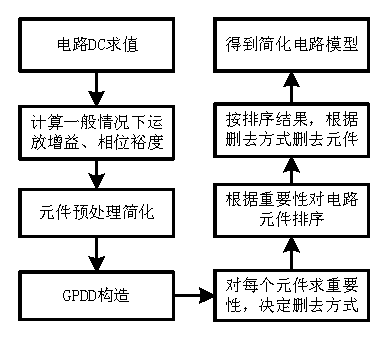
\includegraphics[width=0.5\textwidth]{chap2/SimpProcedure.eps}
	\bicaption[fig:SimpProcedure]{降阶模型自动生成整体流程}{降阶模型自动生成整体流程}{Fig}{Entire procedure for low-order model generation}
\end{figure}

该流程图中有两处以红色斜体标出将在接下来的两个小节\ref{subsec:simp:alg:pre}和\ref{subsec:simp:alg:significance}中详细介绍。
这里先针对其余的部分给出说明。

在拿到一个模拟运放电路后,首先通过数值化仿真器(如:HSPICE)利用DC求解对电路进行求解,以获得电路中所有非线性元件(如:MOSFET)的小信号参数。
接下来,对于完整电路进行AC分析,求得相应的运放增益$A_0$和单位增益频率处相位$PM_0$(即相位裕度处),这两个值将在接下来的元件重要性求值运用到。
对于电路元件进行预处理,做一定粗糙的简化工作,这一步对于生成的最后的简化小信号模型的易于理解性方面有关键的作用,将在\ref{subsec:simp:alg:pre}中具体介绍。
根据初步得到的小信号模型电路,进行GPDD符号化结构的构造,以方便下一步的元件重要性计算。

这里我们定义了电路元件的重要性,某个符号的重要性意味着该电路元件符号对电路性能具有比较大的贡献。
故高重要性的电路元件应予以保留,而低重要性的电路元件应予以删去,故如流程中所示,需要对元件的重要性进行排序。
同时根据前几节的论述,一个符号有两种删去方式,分别为将该元件置为零或无穷大。
我们在计算重要性的过程中即刻确定对应的删去方式,并最终在简化模型生成中以相应的删去方式删去电路元件,从而得到降阶的符号化模型。

这里有一个问题是模型需要多大精度,从而会决定简化的电路模型中保留多少相应的元件。
在目前的研究进程中,我们仅人为指定需要保留多少电路元件,通过人为观察电路频率响应曲线,来决定当前的模型是否合适。

这种简化方法可以看到在符号化构建GPDD后,最关键的时间复杂度主要集中在对元件重要性求值的这一步上。
别的步骤虽然也有一定的时间损耗,但根据我们的实践经验,相比重要性求值步骤来说可以忽略不计。
重要性求值需要对每个电路元件进行计算,故若一个电路中有N个电路元件,构造得到的GPDD结构共有$\left|GPDD\right|$节点。
在\ref{subsec:simp:alg:significance}中可以看到单个元件的重要性求值需$O\left(\left|GPDD\right|\right)$的时间复杂度。
故简化流程的时间复杂度主要由$O\left(N\left|GPDD\right|\right)$决定。

\subsection{元件预处理过程}
\label{subsec:simp:alg:pre}

之所以要对电路进行预先简化,其主要目的在于能够事先将一些信号不通过的节点识别出来,从而事先删去一些节点和元件,方便进一步简化算法。
许多电路从理论上分析,往往会有一定的做法;然而在实际操作中,人们往往会进一步加入自己的理解与分析,从而改变理论分析的结果,虽然过程中隐去了一些电路结构,却使进一步的分析与电路理解更加便利。
这一点在后续的测试结果中也有所体现。
这里以模拟电路中常见的由于输入差分对所造成的虚拟地作为例子,说明这种情况。

\begin{exmp}
虚拟地理论分析与实际操作区别

\begin{figure}[!htp]
	\centering
	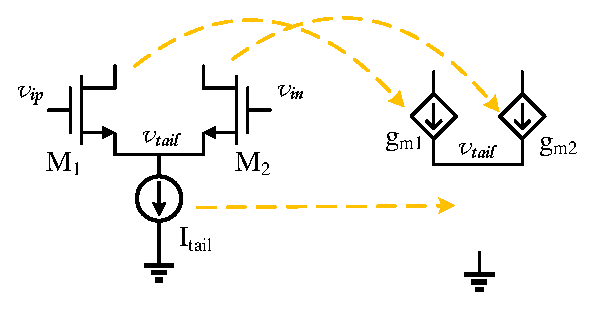
\includegraphics[width=0.6\textwidth]{chap2/VG.eps}
	\bicaption[fig:VG]{虚地的产生原因}{虚地的产生原因}{Fig}{Virtual ground illustration}
\end{figure}

可以看到,图\ref{fig:VG}中展现了经典的模拟电路输入差分对,这样的电路结构一般由一个电流源作为两个输入管的偏置,输入结构两端对称。
在这种结构下,根据传统的电路分析技巧,我们可以画出如图\ref{fig:VG}右侧的小信号结构。
其中理想电流作为断路,所以$v_tail$这一电路节点浮空,同时保留这里的两个MOS管的$g_m$电流源。
我们可以根据$v_tail$这一电路节点的KCL关系,可列写方程有:

\begin{equation}
g_{m1}\left(v_{ip}-v_{tail}\right)+g_{m2}\left(v_{in}-v_{tail}\right)=0
\end{equation}

由于两端的对称性我们知道$v_{ip}=-v_{in}$,并且$g_{m1}=g_{m2}=g_m\neq0$,那么有

\begin{equation}
g_{m} v_{tail} = 0 \Rightarrow v_{tail} = 0
\end{equation}

所以由于尾电流的节点往往被作为虚拟地的存在,在电路分析中往往直接将这一点接到地上,而不是像小信号分析中将电路节点浮空。
这种看似矛盾,实际合理的人为处理结果计算机往往很难自动识别,因为从电路基本理论分析,电路中的电流源应该使用断路的端口进行替代。
即使使用MOS管进行替代,根据传统分析经验,我们知道MOS管往往会近似为一个$r_{ds}$所组成的阻抗,而单一的阻抗并不影响上述分析过程,虚地仍然存在,而往往这个阻抗往往比较大,最后仍然会作为浮空处理。
但这与多数模拟电路工程师的设计经验不符,电路工程师会将类似的结构直接接到地上进行分析。

\end{exmp}

另两种常见的类似电路结构是偏置电路以及镜像电流源。如镜像电流源,往往小信号分析中,作为电流源的MOS管使用电压偏置也并不影响电路的差分工作特性。
造成这种现象的主要原因在于电路信号往往并不直接通过这些节点进行传递,故导致了小信号电路中较低的电压值。
为避免这些电路结构对我们的分析造成影响,我们采取以下的方式对电路进行预处理:

\begin{enumerate}
	\item 求得电路中所有节点的直流处的AC增益。
	\item 将增益最小的节点接地,并删去应删去的元件。(元件的所有端口全接地。)
	\item 如电路的传输相应曲线有较大变化,则终止预处理;否则,回到第2步继续处理。
\end{enumerate}

在这种方案下,我们得到比较合理以及符合工程师习惯的简化电路模型,具体结果可以参照\ref{subsec:simp:res:pre}小节。

\subsection{元件重要性选取}
\label{subsec:simp:alg:significance}

元件重要性是在符号简化工程中十分重要的一个指标。
重要性表征了电路总体性能与某个单一元件的值的密切程度。
如果一个元件的重要性程度高,那么代表电路性能对这个元件的值十分敏感,故在最终的降阶模型电路图中应有所保留。
针对一个运放来说,只有其运放的差分增益以及相位裕度是我们最为关心的两个指标。

\begin{figure}[!htp]
	\centering
	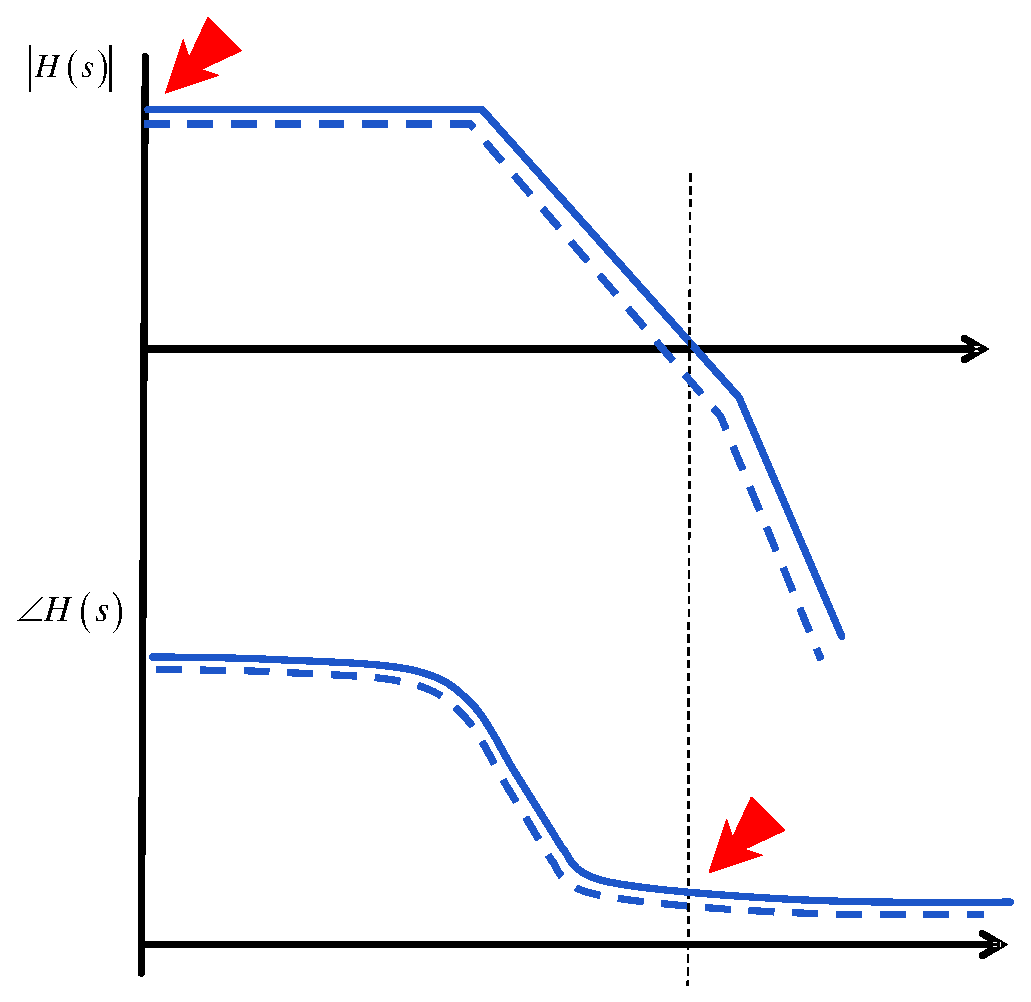
\includegraphics[width=0.7\textwidth]{chap2/significance.eps}
	\bicaption[fig:significance]{元件变化对运放增益和相位裕度的影响}{元件变化对运放增益和相位裕度的影响}{Fig}{The impact of element value on gain and phase margin}
\end{figure}

可以想象,如图\ref{fig:significance},当运放电路元件发生变化的过程中,其相应的差分增益与单位增益频率处的相位会发生变化。
同样,如果一个元件对运放的差分增益贡献较大,那么在把这个元件从电路中以置为无穷大或者零的方式,将其从电路中删去后,电路的频率响应会发生剧烈变动。
也就是说,一个运放的重要性基本等同于元件变化时的电路性能变化的程度。
这一点,正是作为我们选取重要性指标的关键所在。

\begin{figure}[!htp]
	\centering
	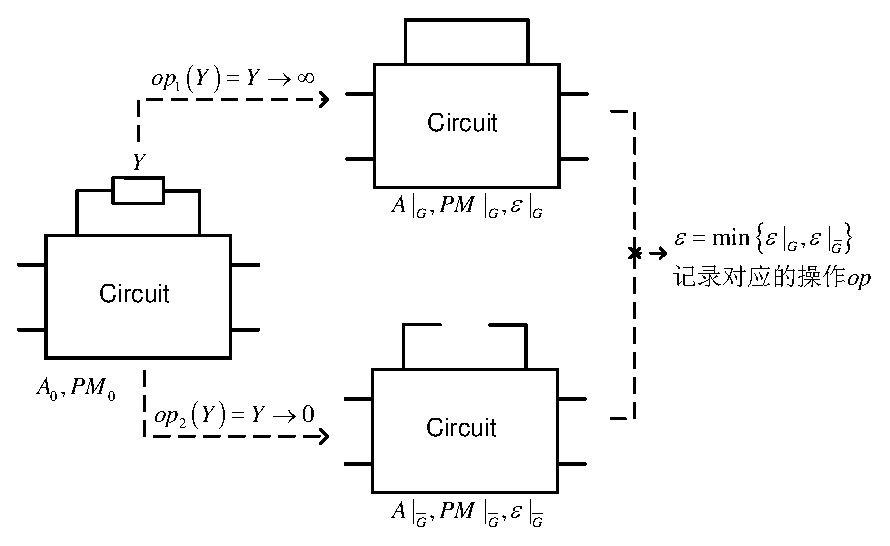
\includegraphics[width=0.8\textwidth]{chap2/SignProcess.eps}
	\bicaption[fig:SignProcess]{元件重要性计算流程}{元件重要性计算流程}{Fig}{Element significance calculation process}
\end{figure}

总结来说,元件重要性计算的整体流程如图\ref{fig:SignProcess}所示。
在算法运行初期,我们得到了运放在一般情况下的差分增益$A_0$以及其在单位频率$UGF$处的相位$PM_0$。
接下来,假设我们需要对电路中的元件$S$求取重要性,那么我们首先将$S$的值置为无穷大,取得此时的运放差分增益$A|_G$以及其在单位频率$UGF$处的相位$PM|_G$,并记录相应的操作为$op1$。
然后,将$S$的值置为零,取得此时的运放差分增益$A|_{\overline G}$以及其在单位频率$UGF$处的相位$PM|_{\overline G}$,并记录相应的操作为$op2$。
在获得了相应的变化之后,我们可以分别计算得到电路在两种情况下分别的电路AC性能的变动指标。
这里我们采用了平方和开根的方式对增益和相位两个指标进行融合。
同时,为了保证两种不同的物理量之间相互能够比较,采用了相对误差的计算方式,如下两式所示:

\begin{equation}
\varepsilon {|_G} = \sqrt {{{\left( {\frac{{A{|_G} - {A_0}}}
				{{{A_0}}}} \right)}^2} + {{\left( {\frac{{PM{|_G} - P{M_0}}}
				{{P{M_0}}}} \right)}^2}}
\end{equation}

\begin{equation}
\varepsilon {|_{\overline G }} = \sqrt {{{\left( {\frac{{A{|_{\overline G }} - {A_0}}}
				{{{A_0}}}} \right)}^2} + {{\left( {\frac{{PM{|_{\overline G }} - P{M_0}}}
				{{P{M_0}}}} \right)}^2}}
\end{equation}

在获得将电路元件置为无穷大和零情况下相应的电路性能的变化$\varepsilon {|_G}$和$\varepsilon {|_{\overline G }}$之后,我们选取其中较小的一个作为之后用于排序的重要性指标$\varepsilon$,同时记得记录对应的删去操作$op$,即如下式:

\begin{equation}
\varepsilon  = \min \left\{ {{\varepsilon {|_G}},{\varepsilon {|_{\overline G }}}} \right\}
\end{equation}

之所以选择较小的$\varepsilon$作为该元件的重要性,主要是因为我们希望在删去电路元件的过程中,应该尽可能小地改变电路的性能指标。
即所选择的$\varepsilon$所对应的删去方式,更适合作为该元件的删去方式,因为删去该元件之后,对电路产生的影响较小。
如有一个电阻,如果其值非常小,可以近似视为短路时,那么明显$\varepsilon {|_G}$会小于$\varepsilon {|_{\overline G }}$,这时应将该电路短路,即选择$\varepsilon {|_G}$作为其重要性,并进行接下来的操作。

可以看到重要性计算过程中需要求取在元件值为零和无穷大时分别的AC增益和$UGF$处的相位,故需要对两种符号情况的两个频率点分别计算电路的传输函数。
这总共需要对GPDD进行4次遍历过程,才可以完成,如忽略常数系数,则重要性计算的时间复杂度约为$\left|GPDD\right|$。

\subsection{简化特殊情况分析}
\label{subsec:simp:alg:special}

在简化过程中,存在两种可能的简化特殊情况,需要区别处理。
出现这些情况的主要原因是对应的电路中拓扑结构不合理造成的。
为了使算法能尽可能稳定运行,在不影响电路性能的情况,尽可能多地删去较多的元件。
应对这些情况做出合适处理,以使算法尽可能稳定。

\subsubsection{元件重要性计算过程中处理}
\label{subsubsec:simp:alg:special:sign}

首先在重要性计算过程中,我们是将电路元件的值置为零或无穷大的情况下,然后计算相应的重要性。
但是有可能出现这样的情况,比如某个电路元件承担了将信号从上一级传递到下一级的职责。
那么我们在计算其重要性过程中,如将其值置为无穷大,那么其输出也为无穷大(在程序中显示其值为INF);
如将其值置为零,那么其输出与输入无关(在程序中显示其值为NAN)。
这两种情况都是我们不期望看到的。所以应规定相应的规则,处理类似情况。我们规定如下规则,处理类似情况:

\begin{enumerate}[label=\emph{\alph*})]
	\item 如没有删去方式会导致对应的重要性$\varepsilon$为INF或者NAN,那么按照\ref{subsec:simp:alg:significance}中的重要性计算方式计算。
	\item 如有仅一种删去方式导致对应的重要性$\varepsilon$为INF或者NAN,那么无论另一种删去方式的重要性$\varepsilon$大小,选择另一种删去方式,并记录重要性。
	\item 如果两种删去方式都会导致对应的重要性$\varepsilon$为INF或者NAN,那么对该元件的操作方式记录为保留,即在后续处理中忽略该元件。
\end{enumerate}

通过这种方式,将有效地避免上述出现的情况。保证算法运行的稳定,尽可能多地删去电路元件,以得到合理的低阶电路模型。

\subsubsection{最终电路图中删去元件过程处理}
\label{subsubsec:simp:alg:special:reduce}

另一种特殊情况发生在最终对电路进行电路图层面的约减过程中。因为在电路图的约减过程中,我们仍然需要监控电路的传输函数变化,来确定最终的小信号简化低阶模型的形式。
有些电路需要多个电路元件删去后,才会出现电路传输函数的计算过程中的异常值(NAN或INF)。
这种情况在GPDD计算中,一种常见的情况是电路出现了孤立节点。
然而由于GPDD的构造过程,是枚举电路生成树对,如果由于简化电路,孤立的节点不会出现生成树中,那么就无法计算对应的GPDD的值。
这种情况往往需要对元件的删去方式进行翻转,因为往往这种情况并不影响最终的传输函数结果。下面用一个例子对这种情况进行说明。

\begin{exmp}
电路中多余元件对GPDD求值的影响
	
\begin{figure}[!htp]
	\centering
	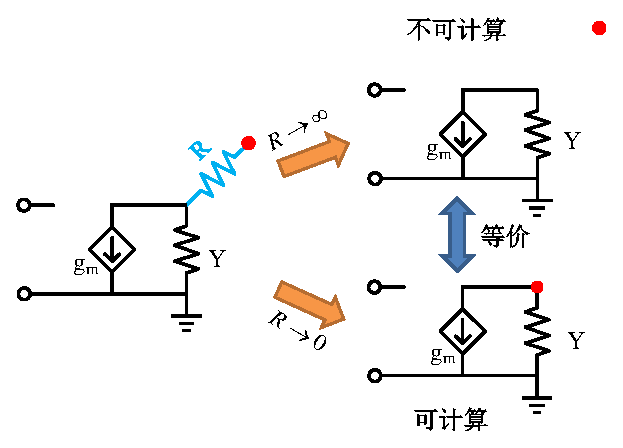
\includegraphics[width=0.6\textwidth]{chap2/CancelCase.eps}
	\bicaption[fig:CancelCase]{电路图约减过程中特殊情况说明}{电路图约减过程中特殊情况说明}{Fig}{Special case in simplified circuit graph reduction}
\end{figure}

可以看到图\ref{fig:CancelCase}中展示了一个多余的电路元件电阻$R$,现在考虑将电阻R删去。
可以看到不论如何删去R都不会影响到电路的传输函数的相应,可是在GPDD中,只有下一种情况是可以继续计算的,因为红色的节点仍然能包含最终的生成树中;
而另一种情况则不包含。这种情况下,GPDD求值存在困难。故如当我们发现类似图\ref{fig:CancelCase}中的情况发生时,及时地改变电路元件的删去方式,那么可以得到可计算的GPDD结构。

\end{exmp}

可以看到只要翻转删去方式,往往可以避免此类的情况的出现;如翻转了仍无效果,可如上一小节\ref{subsubsec:simp:alg:special:sign}中所介绍的一样,保留该元件。
究其深层次的原因,主要是因为GPDD并不完全没有对消项造成的,仍存在类似公因子对消项,这一点会在附录\ref{app:cancel}中给出详细的说明。

\section{降阶模型生成算法测试结果与分析}
\label{sec:simp:res}

\subsection{预处理简化降阶电路模型区别}
\label{subsec:simp:res:pre}

\subsection{多种电路结构简化结果分析}
\label{subsec:simp:res:cir}

\subsubsection{折叠共源共栅运算放大器拓扑简化结果}
\label{subsubsec:simp:res:cir:fd}

\subsubsection{多种补偿结构的两级运算放大器拓扑简化结果}
\label{subsubsec:simp:res:cir:ts}

\subsection{尺寸调整下的算法稳定性分析}
\label{subsec:simp:res:size}

\subsection{简化符号化模型阶数比较}
\label{subsec:simp:res:order}

\section{本章小结}
\label{sec:simp:con}

本章对本文的关键技术符号降阶模型的自动生成进行了详细介绍,并分析了加入各个流程原因以及需要考虑的特殊情况。
通过广泛大量的测试,可以看到本文提出的符号化降阶算法有效地降低了电路模型的阶数,并且得到十分合理、易于电路工程师进行理解的简化电路小信号模型。
这里采用的关键技术为符号化拓扑的简化的方法。这一方法相对于传统的一些符号化简化方法,总结下来,有以下几方面优势:

\begin{enumerate}[label=\emph{\alph*})]
	\item 可以直接给出简化后的电路拓扑结构,易于模拟电路工程师进行分析。
	\item 在过程中,同时得到电路的符号化公式,可直接提供给用户做进一步分析。
	\item 得到的简化结果直接对应于原始电路中的电路元件,有助于做尺寸调整,避免了传统方法中简化结果无法对应会电路的问题。
	\item 区别于传统矩阵降阶方法,是一种启发式的符号化模型降阶方法。
\end{enumerate}
%# -*- coding: utf-8-unix -*-
\chapter{应用一:时域符号化简化模型自动生成方法}
\label{chap:time}

通过上一章的分析,可以看到电路简化模型在频率响应分析上表现出了不错的稳定性与有效性。
本章通过借用前一章分析得到的简化电路模型,尝试构造相应的电路结构,从而得到可以用于时域大信号的电路模型,并通过电路测试结果来显示方法的效果。

\section{传统的时域模型分析方法}
\label{sec:time:origin}

对于传统的运算放大器,其阶跃响应输出往往呈现如图\ref{fig:slewmeaning}所表现的形式。

\begin{figure}[!htp]
	\centering
	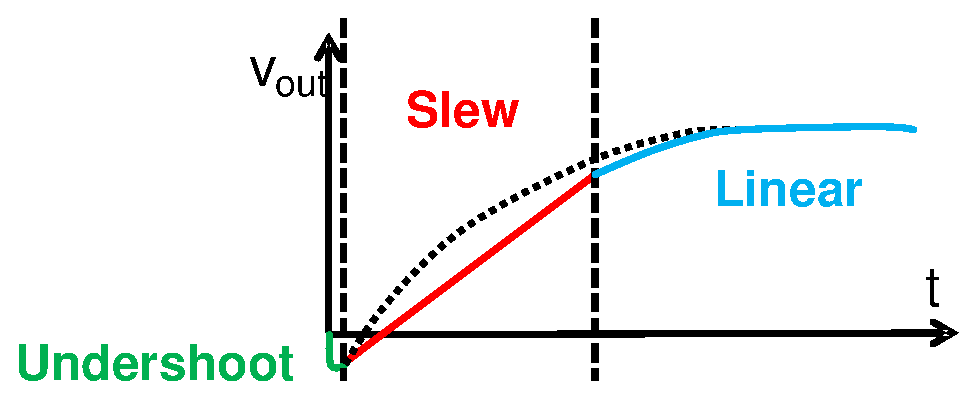
\includegraphics[width=0.6\textwidth]{chap3/SlewMeaning.eps}
	\bicaption[fig:slewmeaning]{Slew-Settling过程}{Slew-Settling过程}{Fig}{Slew-Settling procedure}
\end{figure}

图中,首先绿色部分为Undershoot部分,为线性响应,往往由于运放反馈连接中的零点造成,蓝色部分为Settling过程的线性响应部分。
其中最为关键的是红色的Slew部分。
由于在实际情况中,运放的输出能力有限,不可能输出无限大的电流,所以在运放输出端给输出端所寄生的电容充电的过程中,电压不一定能以线性的工作方式与时间呈指数上升(如黑色虚线所示)。
这种情况下由于电流输出已饱和,基本为以恒定值,故运放输出端电压随时间成比例增长,这条曲线的斜率称之为压摆率(Slew Rate,SR),一般压摆率的估计值可由输出电流$I$与输出端电容$C$的比值决定,如下式所示。

\begin{equation}
SR = \frac{I}{C}
\end{equation}

为了对运放的Slew-Settling过程进行分析,往往需要对运放的这一过程进行建模。
但是由于上述的公式十分粗糙,很难以用于比较精细的电路分析中。
故有大量研究使用各种方法对运放的时域模型进行建模。
\parencite{Pug-3Segment-2010}提出了三段式模型对这一过程进行建模。所谓三段式模型即根据运放响应的三个不同的过程(Undershoot,Slew,Settling)进行分段处理,从而形成一个用于表示运放行为的分段函数作为模型。
\parencite{Yavari-TSSlew-2005,Rezaee-FCSlew-2009}中使用了大信号分析,从电路器件模型出发,通过直接求解电路微分方程等方法对Slew-Settling行为进行分析。
这两种方式虽然有一定处理此类问题的能力,但是相对来说,其公式处理十分繁琐同时由于电路被抽象成一个个分段函数,同时往往需要计算积分等复杂运算,很难回溯会具体的电路器件进行分析,也很难自动化进行。

1982年,Chuang等人提出了在线性系统中加入限制的方式来模拟电路的Slew-Settling模型\parencite{Chuang-Slew-1982}。
这种方法因其本质上是线性系统,仅通过电流的输出能力大小来限制其输出信号,故比较适用与可以分析零极点的符号化方法。
今年来,G. Shi等人通过结合符号化零极点分析与Chuang的电路模型\parencite{ZhangHe-Slew-2011,ZhangAilin-Slew-2015},提出了使用运放宏模型的方式对运放进行建模。
这种方式不仅更为准确,同时提供了更明确的电路意义。一个二级运算放大器的电路宏模型如下图\ref{fig:macromodel}所示:

\begin{figure}[!htp]
	\centering
	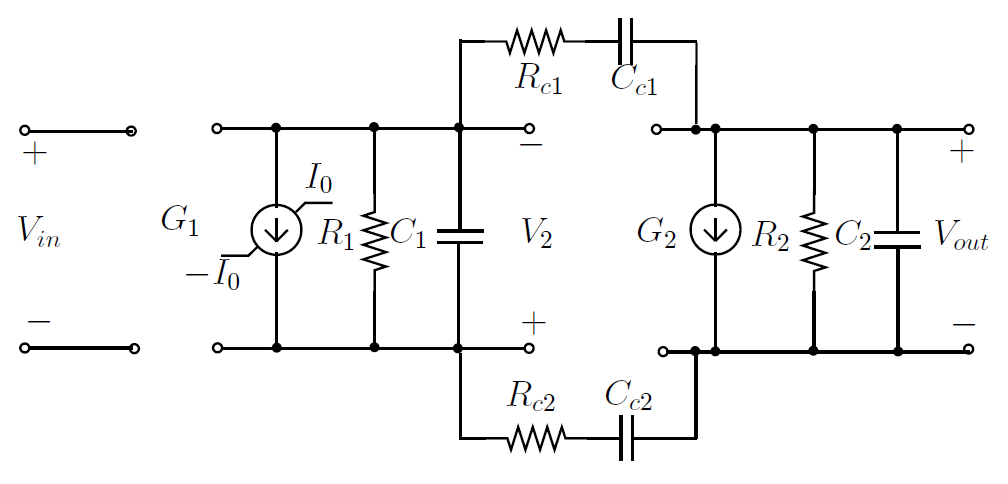
\includegraphics[width=0.6\textwidth]{chap3/macromodel.png}
	\bicaption[fig:macromodel]{运放时域宏模型}{运放时域宏模型\parencite{ZhangAilin-Slew-2015}}{Fig}{Opamp macromodel in time domain\parencite{ZhangAilin-Slew-2015}}
\end{figure}

可以看到通过提取二级运算放大器中各级的零极点,就可以得到每一级中跨导和相应的阻抗与电容。同时注意第一级运放的跨导有电流输出的限制,以模拟运放电路本身的电流输出限制。
那么现在问题就主要在于宏模型电路中各个元件的参数选取上,通过GPDD结构与模比配(Moment Matching)的方法可以得到主要的几阶项,从而得到各级的零极点关系。例如,通过GPDD计算,我们可以得到如下公式:

\begin{equation}
H\left( s \right) = \frac{{N\left( s \right)}}
{{D\left( s \right)}} = \frac{{{b_0}{s^0} + {b_1}{s^1} +  \cdots  + {b_q}{s^q}}}
{{{a_0}{s^0} + {a_1}{s^1} +  \cdots  + {a_r}{s^r}}}
\end{equation}

对上式进行泰勒展开后,可以得到:

\begin{equation}
{H_{ex}}\left( s \right) = {m_0}{s^0} + {m_1}{s^1} + {m_2}{s^2} +  \cdots
\end{equation}

其中系数可以通过联立上述两个公式后,对公式两边多次求导的方式,逐一得到相应的系数,如下式所示。

\begin{align}
& m_0 = \frac{b_0}{a_0} \nonumber \\
& m_1 = \frac{{b_1} - {m_0}{a_1}}{a_0} \nonumber \\
& m_2 = \frac{{b_2} - {m_0}{a_2} - {m_1}{a_1}}{a_0} 
\end{align}

故宏模型电路中的跨导$G$、电阻$R$和电容$C$可以以上公式计算得到。这样就建立起了宏模型与电路实际元件之间的关系,有利于日后对于电路性能优化的进一步分析。
这种方式的主要优势在于直接将电路模型中的零极点与电路元件关系挂上勾,从而电路模型不仅可以在时域,也可以在频域进行计算。
更主要的是这种模型,传统仿真器中可以简单地通过编写网表得到,仿真方便便捷。

\section{符号化时域简化模型分析方法}
\label{sec:time:simp}

\subsection{时域符号化简化流程}
\label{subsec:time:simp:process}

本方法的基本流程类似于Chuang模型,首先获取简化的小信号模型,然后在该小信号模型的基础上加入对输出电流饱和的限制。
但是,本方法与Chuang模型有三点不同,分别为:

\begin{enumerate}[label=\emph{\alph*})]
	\item 简化的小信号零极点模型可以直接通过第二章的符号化模型降阶算法得到。
	\item 限制电流加载运放中所有得以保留的$g_m$元件上,并用大信号中的通过管子的电流作为其限制电流。
	\item 采用了更加光滑的非线性函数,以更加真实地模拟实际情况。
\end{enumerate}

\begin{figure}[!htp]
	\centering
	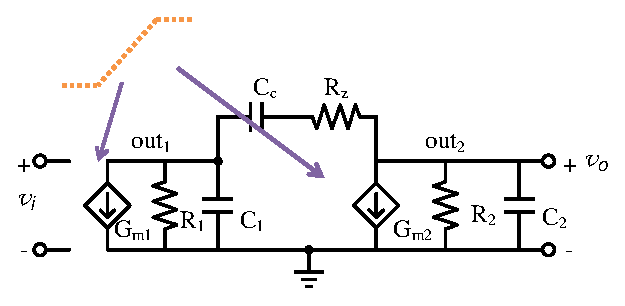
\includegraphics[width=0.6\textwidth]{chap3/CurrentLimitPos.eps}
	\bicaption[fig:limitcur]{时域模型中的电流限制位置}{时域模型中的电流限制位置}{Fig}{Current limit position in slew-settling model}
\end{figure}

其中第一点正是相比之前的方法的闪光点。因为之前的方法,即使是一般的零极点模型,往往很难建立模型与电路元件之间的关系,而给出简化小信号模型可以直观地给出两者之间的联系。

第二点可参考图\ref{fig:limitcur}的示意,本方法将运放电路中所有存在的$g_m$均加入限制。
\parencite{Yavari-TSSlew-2005}中指出,现代的模拟集成电路由于其功耗降低,电源电压降低等原因,造成电流输出饱和的原因不一定是由输入级决定的,可能是之后的电路充电速度不足导致。
Chuang模型中只考虑了第一级电路的输出饱和,对之后级的输出限制没有做出过多考量。
如果在各个$g_m$上加入相应的电流限制,那么即可模拟各级中的电流限制。

\begin{figure}[!htp]
	\centering
	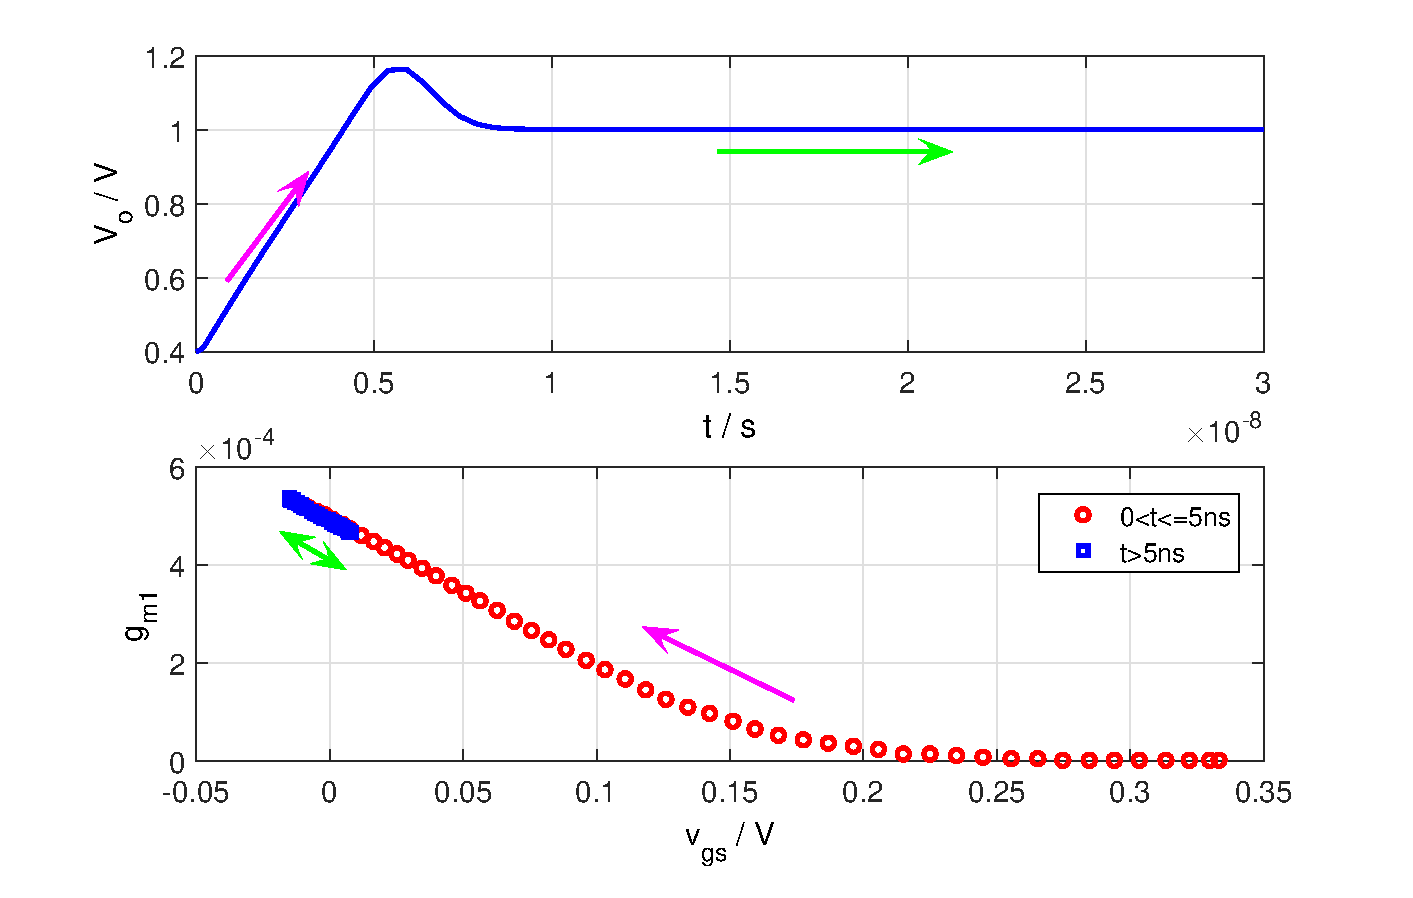
\includegraphics[width=0.8\textwidth]{chap3/gmvariation.eps}
	\bicaption[fig:gmvariation]{Slew-settling过程中输入管$g_m$的变化}{Slew-settling过程中输入管$g_m$的变化}{Fig}{$g_m$ variation during the slew-settling procedure}
\end{figure}

图\ref{fig:gmvariation}给出了两级运算放大器slew-settling的过程中输入管的$g_m$随着输入交流小信号的变化。
图中箭头方向代表了时间的流向。在Slew过程(红色圆圈)中,$g_m$快速爬升至所需要的稳态情况的值;而在Settling过程(蓝色方块)中,$g_m$稳定在某一值不再变化。
以往,我们往往假设$g_m$的函数是一个分段函数,在未饱和前,输入电压和输出电流成正比;饱和后,输出稳定电流。
这样的话$g_m$仅有两个值,其一是稳态情况下的跨导,另一个是$0$。
然而在图中明显看到这样的假设是不合理的,一个办法就是重新决定施加给$g_m$的非线性函数。

\subsection{非线性函数选取}
\label{subsec:time:simp:nonlinear}

非线性函数有许多不同的形式。
一类合适的函数是S型函数族$S_i\left(x\right)$。
这里列举了五种不同的函数方程共参考:
\begin{align}
&{S_0}\left( x \right) = \left\{ {\begin{array}{*{20}{c}}1 & {x \geqslant 1}  \\x & { - 1 \leqslant x < 1}  \\{ - 1} & {x < 1}  \\\end{array} } \right. \\
&{S_1}\left( x \right) = \tanh \left( x \right) \hfill \\
&{S_2}\left( x \right) = \frac{2}{\pi }gd\left( {\frac{\pi }	{2}x} \right) = \frac{2}{\pi }\arcsin \left( {\tanh \left( {\frac{\pi }{2}x} \right)} \right)\\
&{S_3}\left( x \right) = \frac{x}{{\sqrt {1 + {x^2}} }}\\
&{S_4}\left( x \right) = \frac{2}{\pi }\arctan \left( {\frac{\pi }{2}x} \right)
\end{align}

\begin{figure}[!htp]
	\centering
	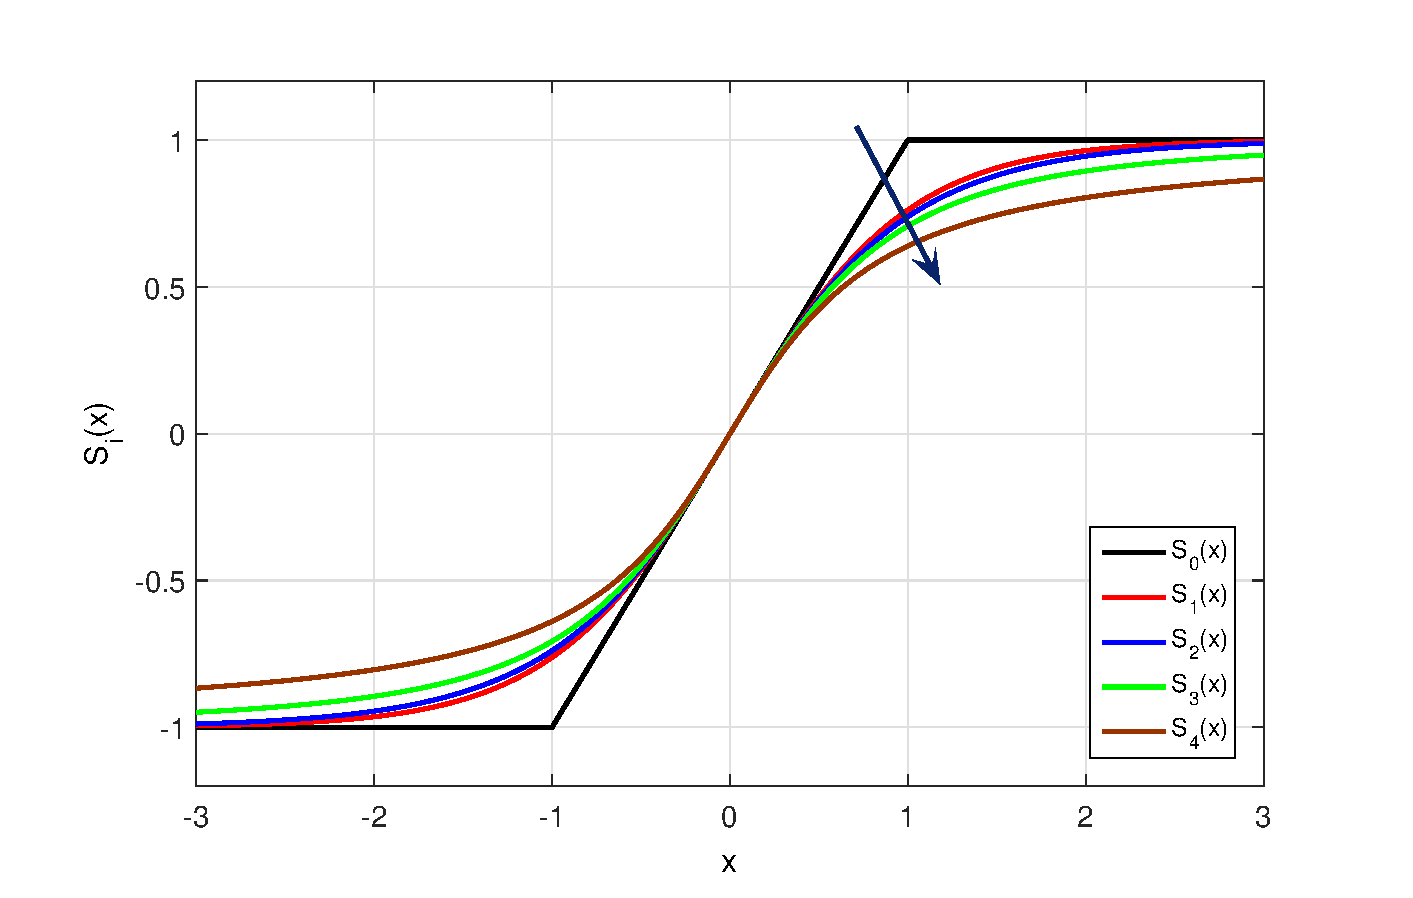
\includegraphics[width=0.8\textwidth]{chap3/sigmoid.eps}
	\bicaption[fig:sigmoid]{S型函数族}{S型函数族}{Fig}{Sigmoid function family}
\end{figure}

图\ref{fig:sigmoid}中展示了所有这5中S型函数的曲线。
可以看到原先在Chuang模型中使用的非线性函数即为这里的$S_0\left(x\right)$。
图中的箭头显示了这些函数在正半平面或负平面中不互相相较,且呈现出了一定顺序。
这类函数有一些共同的特征,如它们都绝对单调递增,可总结如下:

\begin{eqnarray}
\mathop {\lim }\limits_{x \to  + \infty } {S_i}\left( x \right) = 1\\
\mathop {\lim }\limits_{x \to  - \infty } {S_i}\left( x \right) = -1\\
{\left. {\frac{d}{{dx}}{S_i}\left( x \right)} \right|_{x = 0}} = 1
\end{eqnarray}

如果有一个跨导的DC偏置电流是$I_0$,其增益为$g_m$,那么对这类函数只需要做如下的变换即可得到我们所需要的非线性的$g_m$。

\begin{equation}
{I_0}{S_i}\left( {\frac{{{g_m}}}{{{I_0}}}x} \right)
\end{equation}

\section{符号化时域简化模型分析方法}
\label{sec:time:test}

\subsection{两级运放测试结果}
\label{subsec:time:test:ts}

\begin{figure}[!htp]
	\centering
	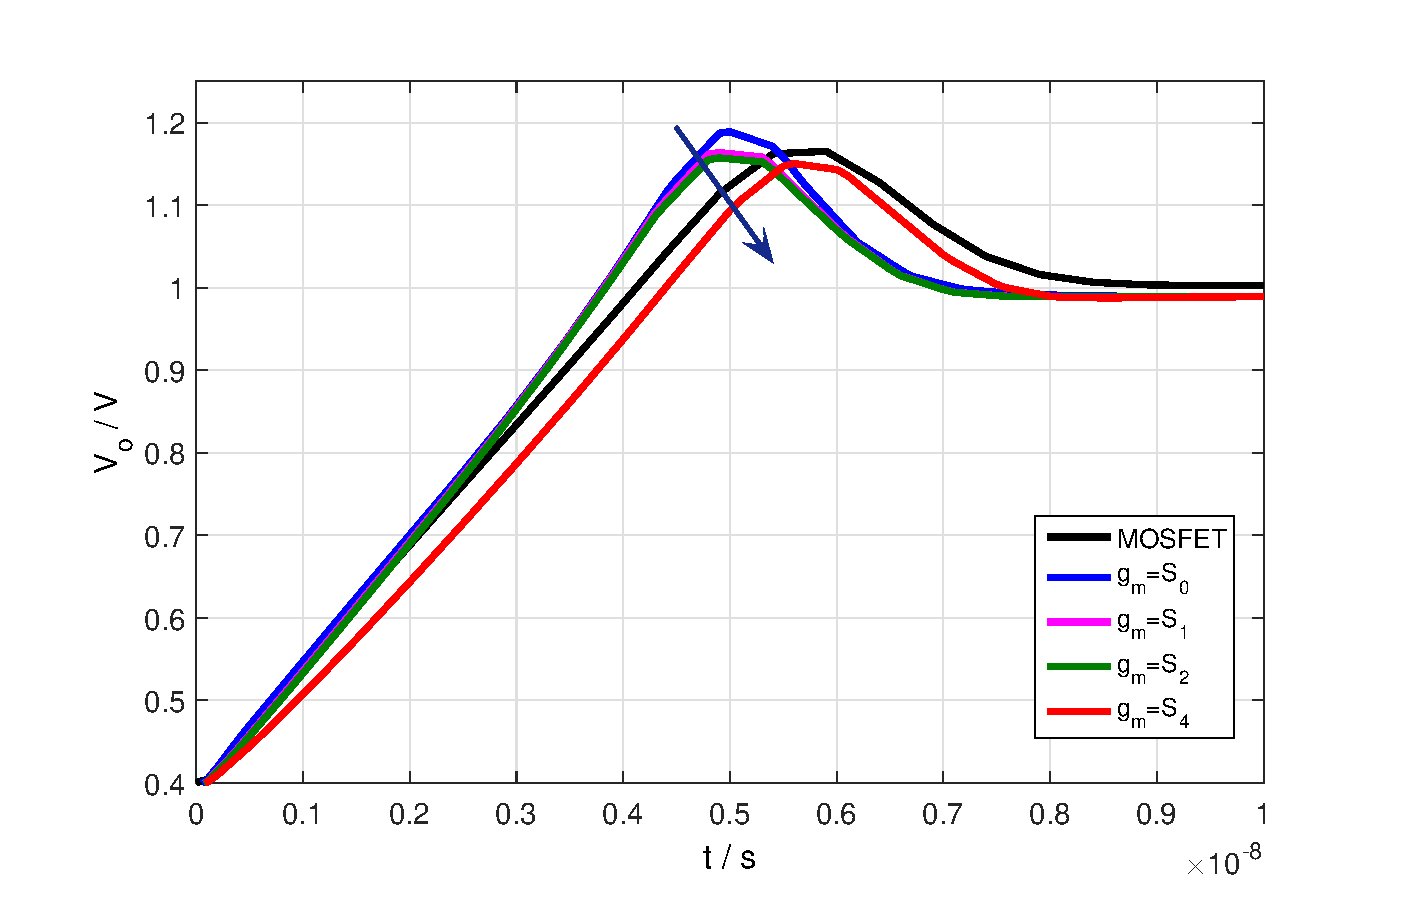
\includegraphics[width=0.8\textwidth]{chap3/TS_Slew.eps}
	\bicaption[fig:tsslew]{两级运放模型的Slew-Settling时域仿真结果}{两级运放模型的Slew-Settling时域仿真结果}{Fig}{Simulation Results of slew-settling behavior for two-stage opamp model}
\end{figure}

首先我们针对两级运放电路进行了电路时域模型的建模,图\ref{fig:tsslew}中展示了在不同S型函数作用下的电路的Slew-Settling行为。
可以看到$S_0\left(x\right)$、$S_1\left(x\right)$和$S_2\left(x\right)$在Slew阶段表现出了良好的对压摆率的估计行为。
而$S_4\left(x\right)$则非常适于对于电路稳定时间的估计。
这里并没有画出相应的$S_3\left(x\right)$的曲线,因为其HSPICE仿真并不收敛。
可以发现图中的箭头标志了这些函数作用下的时域曲线也呈现了一定的顺序,且与上一小节中的次序一致。
故可以预估$S_3\left(x\right)$会取得最好的电路近似程度。

\subsection{折叠共源共栅运放测试结果}
\label{subsec:time:test:fc}

在对折叠共源共栅运放的电路测试中,我们发现只有$S_1\left(x\right)$的作用下,电路才可以顺利由HSPICE求解出来,仿真结果如图\ref{fig:fcslew}。
这里结果十分值得怀疑,因为其中出现了奇怪的折角,这在电路稳定的情况下不应该出现。
同时,此时本方法生成的时域运放模型并不能很好地抓取电路的时域特性,说明时域模型生成方法仍存在一些问题,需要进一步分析验证。

\begin{figure}[!htp]
	\centering
	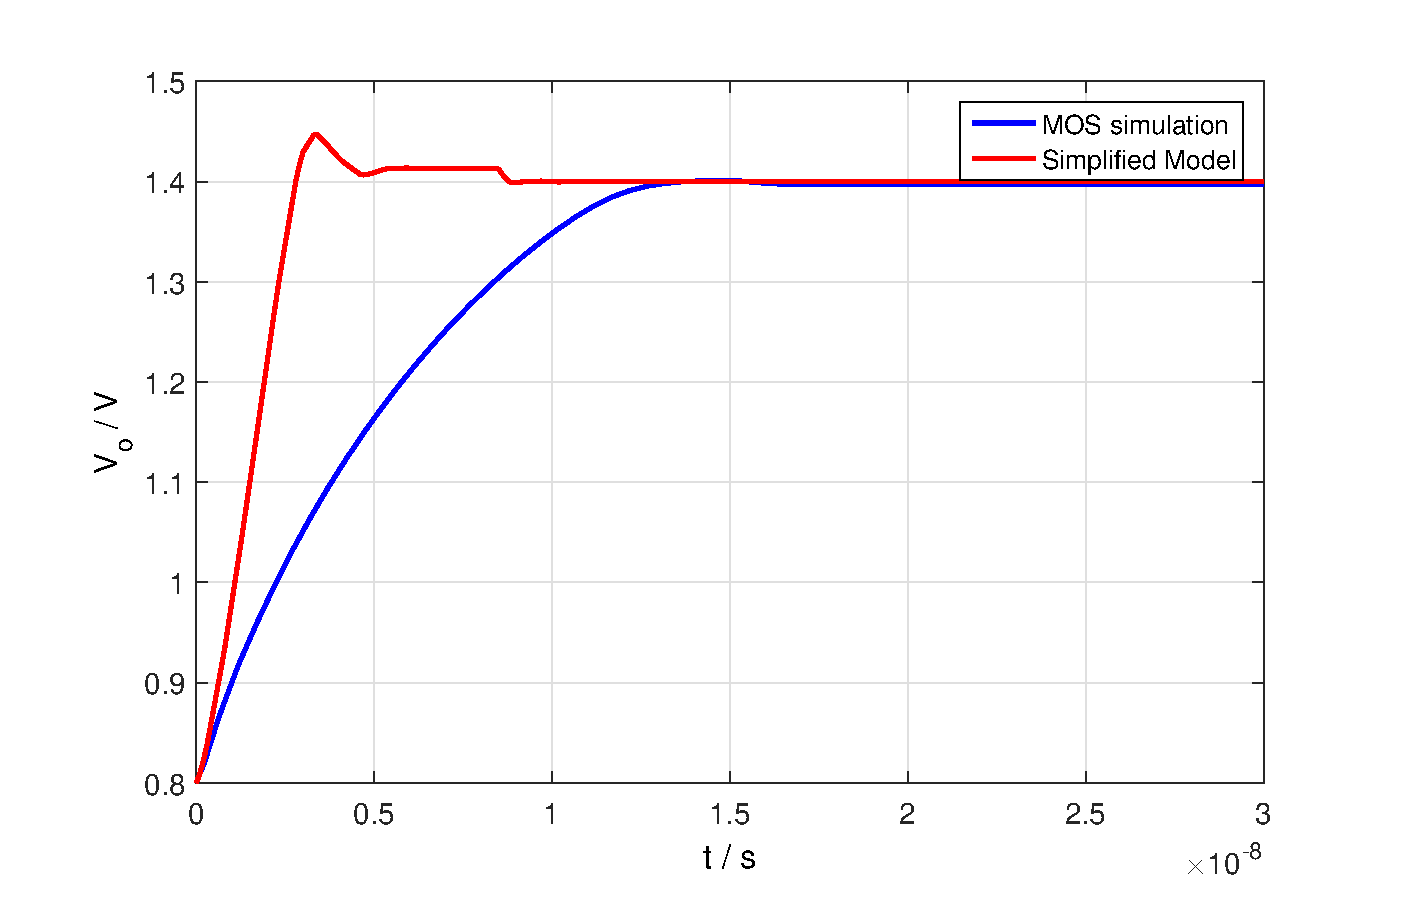
\includegraphics[width=0.8\textwidth]{chap3/FC_Slew.eps}
	\bicaption[fig:fcslew]{折叠共源共栅运放模型的Slew-Settling时域仿真结果}{折叠共源共栅运放模型的Slew-Settling时域仿真结果}{Fig}{Simulation Results of slew-settling behavior for folded-cascode opamp model}
\end{figure}

\section{本章小结}
\label{sec:time:con}

本章主要回顾了时域模型生成方法的相关历史,并提出了自己的时域模型简化方法,并对方法进行了测试。
这种方法的优势在于其生成的模型是符号化的,并且大部分流程可以自动化,不需要过多的电路经验也可以对电路模型进行分析。
可以看到目前符号化时域简化模型分析方法仅针对部分电路可以成功使用,但是仍有许多电路存在分析困难的情况。
需要进一步通过非线性函数选取和系统层面理论分析对电路模型生成的方法进行论证。
%# -*- coding: utf-8-unix -*-
%%==================================================
%% conclusion.tex for SJTUThesis
%% Encoding: UTF-8
%%==================================================

\begin{summary}

这里是全文总结内容。

2015年2月28日,中央在北京召开全国精神文明建设工作表彰暨学雷锋志愿服务大会,公布全国文明城市(区)、文明村镇、文明单位名单。上海交通大学荣获全国文明单位称号。         

全国文明单位这一荣誉是对交大人始终高度重视文明文化工作的肯定,是对交大长期以来文明创建工作成绩的褒奖。在学校党委、文明委的领导下,交大坚持将文明创建工作纳入学校建设世界一流大学的工作中,全体师生医护员工群策群力、积极开拓,落实国家和上海市有关文明创建的各项要求,以改革创新、科学发展为主线,以质量提升为目标,聚焦文明创建工作出现的重点和难点,优化文明创建工作机制,传播学校良好形象,提升社会美誉度,显著增强学校软实力。2007至2012年间,上海交大连续三届荣获“上海市文明单位”称号,成为创建全国文明单位的新起点。         

上海交大自启动争创全国文明单位工作以来,凝魂聚气、改革创新,积极培育和践行社会主义核心价值观。坚持统筹兼顾、多措并举,将争创全国文明单位与学校各项中心工作紧密结合,着力构建学校文明创建新格局,不断提升师生医护员工文明素养,以“冲击世界一流大学汇聚强大精神动力”为指导思想,以“聚焦改革、多元推进、以评促建、丰富内涵、彰显特色”为工作原则,并由全体校领导群策领衔“党的建设深化、思想教育深入、办学成绩显著、大学文化丰富、校园环境优化、社会责任担当”六大板块共28项重点突破工作,全面展现近年来交大文明创建工作的全貌和成就。         

进入新阶段,学校将继续开拓文明创建工作新格局,不断深化工作理念和工作实践,创新工作载体、丰富活动内涵、凸显创建成效,积极服务于学校各项中心工作和改革发展的大局面,在上级党委、文明委的关心下,在学校党委的直接领导下,与时俱进、开拓创新,为深化内涵建设、加快建成世界一流大学、推动国家进步和社会发展而努力奋斗!       

上海交通大学医学院附属仁济医院也获得全国文明单位称号。      

\end{summary}


\appendix	% 使用英文字母对附录编号,重新定义附录中的公式、图图表编号样式
\renewcommand\theequation{\Alph{chapter}--\arabic{equation}}	
\renewcommand\thefigure{\Alph{chapter}--\arabic{figure}}
\renewcommand\thetable{\Alph{chapter}--\arabic{table}}
\renewcommand\thealgorithm{\Alph{chapter}--\arabic{algorithm}}

%% 附录内容,本科学位论文可以用翻译的文献替代。
%# -*- coding: utf-8-unix -*-
\chapter{搭建模板编译环境}

\section{安装TeX发行版}

\subsection{Mac OS X}

Mac用户可以从MacTeX主页\footnote{\url{https://tug.org/mactex/}}下载MacTeX 2015。
也可以通过brew包管理器\footnote{\url{http://caskroom.io}}安装MacTeX 2015。

\begin{lstlisting}[basicstyle=\small\ttfamily, numbers=none]
brew cask install mactex
\end{lstlisting}

\subsection{Linux}

建议Linux用户使用TeXLive主页\footnote{\url{https://www.tug.org/texlive/}}的脚本来安装TeXLive 2015。
以下命令将把TeXLive发行版安装到当前用户的家目录下。
若计划安装一个供系统上所有用户使用的TeXLive,请使用root账户操作。

\begin{lstlisting}[basicstyle=\small\ttfamily, numbers=none]
wget http://mirror.ctan.org/systems/texlive/tlnet/install-tl-unx.tar.gz
tar xzvpf install-tl-unx.tar.gz
cd install-tl-20150411/
./install-tl
\end{lstlisting}

\section{安装中文字体}

\subsection{Mac OS X、Deepin}

Mac和Deepin用户双击字体文件即可安装字体。

\subsection{RedHat/CentOS用户}

RedHat/CentOS用户请先将字体文件复制到字体目录下,调用fc-cache刷新缓存后即可在TeXLive中使用新字体。

\begin{lstlisting}[basicstyle=\small\ttfamily, numbers=none]
mkdir ~/.fonts
cp *.ttf ~/.fonts				# 当前用户可用新字体
cp *.ttf /usr/share/fonts/local/	# 所有用户可以使用新字体
fc-cache -f
\end{lstlisting}


%# -*- coding: utf-8-unix -*-
%% app2.tex for SJTU Master Thesis
%% based on CASthesis
%% modified by wei.jianwen@gmail.com
%% version: 0.3a
%% Encoding: UTF-8
%% last update: Dec 5th, 2010
%%==================================================

\chapter{Maxwell Equations}

选择二维情况,有如下的偏振矢量:
\begin{subequations}
  \begin{eqnarray}
    {\bf E}&=&E_z(r,\theta)\hat{\bf z} \\
    {\bf H}&=&H_r(r,\theta))\hat{ \bf r}+H_\theta(r,\theta)\hat{\bm
      \theta}
  \end{eqnarray}
\end{subequations}
对上式求旋度:
\begin{subequations}
  \begin{eqnarray}
    \nabla\times{\bf E}&=&\frac{1}{r}\frac{\partial E_z}{\partial\theta}{\hat{\bf r}}-\frac{\partial E_z}{\partial r}{\hat{\bm\theta}}\\
    \nabla\times{\bf H}&=&\left[\frac{1}{r}\frac{\partial}{\partial
        r}(rH_\theta)-\frac{1}{r}\frac{\partial
        H_r}{\partial\theta}\right]{\hat{\bf z}}
  \end{eqnarray}
\end{subequations}
因为在柱坐标系下,$\overline{\overline\mu}$是对角的,所以Maxwell方程组中电场$\bf E$的旋度:
\begin{subequations}
  \begin{eqnarray}
    &&\nabla\times{\bf E}=\mathbf{i}\omega{\bf B} \\
    &&\frac{1}{r}\frac{\partial E_z}{\partial\theta}{\hat{\bf
        r}}-\frac{\partial E_z}{\partial
      r}{\hat{\bm\theta}}=\mathbf{i}\omega\mu_rH_r{\hat{\bf r}}+\mathbf{i}\omega\mu_\theta
    H_\theta{\hat{\bm\theta}}
  \end{eqnarray}
\end{subequations}
所以$\bf H$的各个分量可以写为:
\begin{subequations}
  \begin{eqnarray}
    H_r=\frac{1}{\mathbf{i}\omega\mu_r}\frac{1}{r}\frac{\partial
      E_z}{\partial\theta } \\
    H_\theta=-\frac{1}{\mathbf{i}\omega\mu_\theta}\frac{\partial E_z}{\partial r}
  \end{eqnarray}
\end{subequations}
同样地,在柱坐标系下,$\overline{\overline\epsilon}$是对角的,所以Maxwell方程组中磁场$\bf H$的旋度:
\begin{subequations}
  \begin{eqnarray}
    &&\nabla\times{\bf H}=-\mathbf{i}\omega{\bf D}\\
    &&\left[\frac{1}{r}\frac{\partial}{\partial
        r}(rH_\theta)-\frac{1}{r}\frac{\partial
        H_r}{\partial\theta}\right]{\hat{\bf
        z}}=-\mathbf{i}\omega{\overline{\overline\epsilon}}{\bf
      E}=-\mathbf{i}\omega\epsilon_zE_z{\hat{\bf z}} \\
    &&\frac{1}{r}\frac{\partial}{\partial
      r}(rH_\theta)-\frac{1}{r}\frac{\partial
      H_r}{\partial\theta}=-\mathbf{i}\omega\epsilon_zE_z
  \end{eqnarray}
\end{subequations}
由此我们可以得到关于$E_z$的波函数方程:
\begin{eqnarray}
  \frac{1}{\mu_\theta\epsilon_z}\frac{1}{r}\frac{\partial}{\partial r}
  \left(r\frac{\partial E_z}{\partial r}\right)+
  \frac{1}{\mu_r\epsilon_z}\frac{1}{r^2}\frac{\partial^2E_z}{\partial\theta^2}
  +\omega^2 E_z=0
\end{eqnarray}

%# -*- coding: utf-8-unix -*-
\chapter{从 \CJKLaTeX 转向 \XeTeX }
\label{chap:whydvipdfm}

我习惯把v0.2a使用dvipdfmx编译的硕士学位论文模板称为“ \CJKLaTeX 模板”,而这个使用 \XeTeX 引擎(xelatex程序)处理的模板则被称为“{\XeTeX/\LaTeX}模板”。
从 \CJKLaTeX 模板迁移到{\XeTeX\LaTeX}模板的好处有下:
\begin{enumerate}
\item[\large\smiley] 搭建 \XeTeX 环境比搭建 \CJKLaTeX 环境更容易;
\item[\large\smiley] 更简单的字体控制;
\item[\large\smiley] 完美支持PDF/EPS/PNG/JPG图片,不需要“bound box(.bb)”文件;
\item[\large\smiley] 支持OpenType字体的复杂字型变化功能;
\end{enumerate}

当然,这也是有代价的。由于 \XeTeX 比较新,在我看来,使用 \XeTeX 模板所必须付出的代价是:

\begin{enumerate}
\item[\large\frownie] 必须把你“古老的” \TeX 系统更新为较新的版本。TeXLive 2012和CTeX 2.9.2能够编译这份模板,而更早的版本则无能为力。
\item[\large\frownie] 需要花一些时间把你在老模板上的工作迁移到新模板上。
\end{enumerate}

第一条就看你如何取舍了,新系统通常意味着更好的兼容性,值得升级。而转换模板也不是什么特别困难的事情,可以这样完成:

\begin{enumerate}
\item 备份你要转换的源文件,以防你的工作成果丢失;
\item 将你原来的tex以及bib文件另存为UTF-8编码的文件。iconv、vim、emacs、UEdit等等工具都可以完成。WinEdt对文件编码识别功能很差(到了v6.0还是如此),不推荐作为字符编码转换工具;
\item 将diss.tex导言区中的内容替换为XeTeX模板diss.tex导言区的内容;
\item 将你对原先导言区的修改,小心翼翼地合并到新的导言区中;
\item 使用XeTeX模板中的GBT7714-2005NLang.bst替换原有的bst文件,新的bst文件只是将字符编码转换为UTF-8;
\item 删除bouding box文件;
\item 使用本文\ref{sec:process}介绍的方法,重新编译文档;
\end{enumerate}


%# -*- coding: utf-8-unix -*-
\chapter{模板更新记录}
\label{chap:updatelog}

\textbf{2015年6月19日} v0.9发布,适配ctex 2.x宏包,需要使用TeXLive 2015编译。

\textbf{2015年3月15日} v0.8发布,使用biber/biblatex组合替代 \BibTeX ,带来更强大稳定的参考文献处理能力;添加enumitem宏包增强列表环境控制能力;完善宏包文字描述。

\textbf{2015年2月15日} v0.7发布,增加盲审选项,调用外部工具插入扫描件。

\textbf{2015年2月14日} v0.6.5发布,修正一些小问题,缩减git仓库体积,仓库由sjtu-thesis-template-latex更名为SJTUThesis。

\textbf{2014年12月17日} v0.6发布,学士、硕士、博士学位论文模板合并在了一起。

\textbf{2013年5月26日} v0.5.3发布,更正subsubsection格式错误,这个错误导致如"1.1 小结"这样的标题没有被正确加粗。

\textbf{2012年12月27日} v0.5.2发布,更正拼写错误。在diss.tex加入ack.tex。

\textbf{2012年12月21日} v0.5.1发布,在 \LaTeX 命令和中文字符之间留了空格,在Makefile中增加release功能。

\textbf{2012年12月5日} v0.5发布,修改说明文件的措辞,更正Makefile文件,使用metalog宏包替换xltxtra宏包,使用mathtools宏包替换amsmath宏包,移除了所有CJKtilde(\verb+~+)符号。

\textbf{2012年5月30日} v0.4发布,包含交大学士、硕士、博士学位论文模板。模板在\href{https://github.com/weijianwen/sjtu-thesis-template-latex}{github}上管理和更新。

\textbf{2010年12月5日} v0.3a发布,移植到 \XeTeX/\LaTeX 上。

\textbf{2009年12月25日} v0.2a发布,模板由CASthesis改名为sjtumaster。在diss.tex中可以方便地改变正文字号、切换但双面打印。增加了不编号的一章“全文总结”。
添加了可伸缩符号(等号、箭头)的例子,增加了长标题换行的例子。

\textbf{2009年11月20日} v0.1c发布,增加了Linux下使用ctex宏包的注意事项、.bib条目的规范要求,
修正了ctexbook与listings共同使用时的断页错误。

\textbf{2009年11月13日} v0.1b发布,完善了模板使用说明,增加了定理环境、并列子图、三线表格的例子。

\textbf{2009年11月12日} 上海交通大学硕士学位论文 \LaTeX 模板发布,版本0.1a。



\backmatter	% 文后无编号部分 

%% 参考资料
\printbibliography[heading=bibintoc]

%% 致谢、发表论文、申请专利、参与项目、简历
%% 用于盲审的论文需隐去致谢、发表论文、申请专利、参与的项目
\makeatletter
\ifsjtu@review\relax\else
  %# -*- coding: utf-8-unix -*-
\begin{thanks}

  感谢所有测试和使用交大学位论文 \LaTeX 模板的同学!

  感谢那位最先制作出博士学位论文 \LaTeX 模板的交大物理系同学!

  感谢William Wang同学对模板移植做出的巨大贡献!

\end{thanks}
 	  %% 致谢
  %# -*- coding: utf-8-unix -*-
%%==================================================
%% pub.tex for SJTUThesis
%% Encoding: UTF-8
%%==================================================

\begin{publications}{99}
	\item Hanbin Hu, Guoyong Shi, Andy Tai, and Frank Lee, "Topological symbolic simplification for analog design," in \textit{Proc. IEEE Int'l Symposium on Circuits and Systems (ISCAS)}, 2015, pp. 2644-2647.
    \item Hanbin Hu, Guoyong Shi, and Yan Zhu, "Incremental symbolic construction for topological modeling of analog circuits," in \textit{Proc. IEEE Int'l Conf. on ASIC (ASICON)}, 2013, pp. 1-4.
\end{publications}
	  %% 发表论文
% %# -*- coding: utf-8-unix -*-
\begin{patents}{99}
    \item 第一发明人,“永动机”,专利申请号202510149890.0
\end{patents}
	  %% 申请专利
% %# -*- coding: utf-8-unix -*-
%%==================================================
%% projects.tex for SJTUThesis
%% Encoding: UTF-8
%%==================================================

\begin{projects}{99}
    \item 973项目“XXX”
    \item 自然基金项目“XXX”
    \item 国防项目“XXX”
\end{projects}
  %% 参与的项目
% \include{tex/resume}	  %% 各人简历
\fi
\makeatother

\end{document}
